%%
%% Standalone chapter template derived from the full thesis document.
%% Compile this file to work on a single chapter with the Thesis.cls style.
%%
\documentclass[a4paper,11pt,oneside]{Thesis}

% Figures can live next to this file or anywhere else; adjust as needed.
\graphicspath{{Figures/}}

% Match the package setup from the full thesis template.
\usepackage[square, numbers, comma, sort&compress]{natbib}
\usepackage{verbatim}
\usepackage{vector}
\usepackage{lipsum}
\hypersetup{urlcolor=blue, colorlinks=true}

% Optional metadata (kept simple so this stays stripped down).
\title{Standalone Chapter Title}
\authors{Author Name}
\date{\today}

\begin{document}

% The full template uses roman numerals and extensive front matter.
% Here we jump directly into the body content.
\mainmatter
\setstretch{1.3}
\pagestyle{fancy}
\fancyhead{}
\rhead{\thepage}
\lhead{}

% \chapter{Introduction}
% Placeholder content for Chapter 1.
% Chapter 1: Introduction
% \lipsum[1]
% =========================================================
% Chapter 1: Introduction (Lean Draft)
% =========================================================

\chapter{Introduction}
\label{ch:introduction}

\section{Background and Problem Statement}
Object detection is a central problem in computer vision, underpinning practical systems in domains such as transportation, infrastructure monitoring, robotics, and scene understanding. The task requires models to simultaneously recognise object categories and localise them precisely in complex visual environments. Over the past decade, detection performance has advanced rapidly through Convolutional Neural Networks (CNNs) and their multi-scale extensions, enabling strong results on benchmarks and early deployments in the real world. More recently, Vision Transformers (ViTs) and Detection Transformers (DETRs) have emerged as a new paradigm for object detection, offering global context modelling, simplified pipelines, and improved scalability compared to traditional region- or anchor-based detectors.

Despite their promise, DETR-style detectors remain challenging to deploy in real-world settings. Existing variants often incur high computational cost, slower inference, and large data requirements, while exhibiting sensitivity to domain shift and inconsistent performance across object scales. These limitations become particularly pronounced when objects are small, visually subtle, or appear under cluttered or dynamically changing conditions. Consequently, there is a need to better understand the behaviours of DETR models in practice, and to develop architectures that are simultaneously robust, efficient, and explainable beyond controlled benchmark environments.

\section{Motivation}
This thesis is motivated by two converging observations. First, empirical evidence from real-world detection tasks suggests that ViT-based detectors can better represent fine-grained structure and subtle visual patterns than CNN-only pipelines, especially for small or irregular objects. However, directly integrating ViT backbones into multi-scale DETR encoders can substantially increase compute and memory costs, limiting their practicality in efficient or real-time settings. Second, while DETR architectures have grown rapidly in capability, their internal reasoning remains relatively opaque, and systematic explainability studies for DETR variants lag behind those for ViT classifiers. Without clear interpretability and diagnostic tools, architectural weaknesses are difficult to isolate, and design improvements are often guided by trial-and-error.

Together, these observations motivate the central direction of this thesis: to develop \emph{pure Vision Transformer} detection architectures that fuse multi-scale ViT features efficiently, and to use explainability-driven analysis to uncover and address the limitations of Detection Transformers in real-world conditions.

\section{Research Objectives and Questions}
The overarching objective of this research is to investigate the limitations of Detection Transformers in practice, and to design efficient and explainable ViT-based DETR architectures that generalise robustly across diverse environments. Specifically, this thesis addresses the following research questions:

\begin{itemize}
    \item \textbf{RQ1:} What specific challenges do Detection Transformers face in practical applications, particularly regarding real-time processing constraints, varying object scales, and generalisation under domain shift?
    \item \textbf{RQ2:} How can explainability techniques be applied to systematically uncover the decision-making process and identify architectural limitations of Detection Transformers across diverse environments?
    \item \textbf{RQ3:} What architectural modifications can be introduced to Detection Transformers to improve robustness, efficiency, and explainability, especially for multi-scale and small-object detection under real-world conditions?
\end{itemize}

\section{Thesis Contributions}
This thesis makes the following contributions toward efficient and explainable ViT-based object detection:

\begin{itemize}
    \item \textbf{Real-world empirical motivation:} A comprehensive case study on automated road damage detection evaluates CNN and DETR families under domain shift and scale imbalance, demonstrating the potential of ViT-based DETRs for fine-grained and small-object detection.
    \item \textbf{Explainability-driven analysis:} A detailed deconstruction of DETR, Deformable-DETR, and DINO reveals consistent reasoning patterns, attention behaviours, and failure modes, establishing explainability as a diagnostic tool for detector design.
    \item \textbf{ViT-friendly multi-scale fusion:} The proposed \textbf{MCAF-DETR} architecture introduces a multi-scale deformable cross-attention encoder for efficient fusion of hierarchical ViT features, enabling strong multi-scale detection without heavy self-attention encoders.
    \item \textbf{Latent-space decoding for efficiency (forward-looking):} The \textbf{BLCA} framework explores a compact latent workspace for bidirectional query–feature interaction, reducing decoder cost while preserving global–local reasoning capacity.
    \item \textbf{A unified perspective on robust transformer detection:} The thesis consolidates empirical findings and architectural insights into practical guidelines for building efficient, explainable Detection Transformers with pure ViT backbones.
\end{itemize}

\section{Thesis Organisation}
The remainder of this thesis is structured into seven chapters.

\textbf{Chapter~2} surveys object detection foundations, tracing the evolution from CNN-based detectors to ViT and DETR families. It reviews multi-scale modelling strategies and explainability methods that underpin later chapters.

\textbf{Chapter~3} presents a real-world case study on automated road damage detection. Through extensive evaluation across datasets and detector families, it highlights practical challenges in scale imbalance, annotation inconsistency, and domain shift, and motivates ViT-based DETR designs.

\textbf{Chapter~4} provides a comprehensive explainability and failure-case analysis of DETR variants, including Deformable-DETR and DINO. It examines encoder–decoder attention, reference-point dynamics, and scale-dependent errors to identify core architectural limitations.

\textbf{Chapter~5} introduces \textbf{MCAF-DETR}, a ViT-friendly Detection Transformer that replaces CNN feature pyramids with multi-scale deformable cross-attention. The chapter details the architecture, training, and evaluation on MS COCO, demonstrating improved robustness and competitive efficiency.

\textbf{Chapter~6} (optional) proposes \textbf{Bidirectional Latent Cross Attention (BLCA)}, a forward-looking latent-driven decoder framework for efficient DETR-style detection. It outlines the design rationale and early empirical results, and positions the approach for future extension.

Finally, \textbf{Chapter~7} concludes the thesis by summarising key findings, reflecting on limitations, and outlining future research directions for efficient and explainable Vision Transformer detectors.

% =========================================================
% End of Chapter 1 draft
% =========================================================

% TODO: Add References / citations

% \chapter{Literature Review}
% Placeholder content for Chapter 2.
% \lipsum[2]
\chapter{Literature Review}

\noindent
This chapter reviews the foundations and recent advances in object detection with a focus on Vision Transformer (ViT)–based architectures and Detection Transformers (DETR). The aim is to provide the conceptual and technical background necessary to situate the contributions of this thesis within the broader landscape of modern detection research. The chapter begins by outlining the evolution of object detection, from classical feature-driven methods to deep learning–based CNN detectors, highlighting their core assumptions and limitations. It then introduces Vision Transformers and their representational properties, establishing the motivation for transformer-based detection frameworks.

A substantial portion of the chapter examines DETR and its derivatives, tracing the architectural innovations that address DETR’s well-known challenges in convergence, multi-scale reasoning, and small-object performance. The discussion extends to multi-scale modelling strategies, ViT-based DETR variants, and emerging pure-ViT detection pipelines. In parallel, the chapter surveys explainability methods for transformers, noting the scarcity of interpretability studies for DETR and the implications this has for analysing model behaviour. The chapter concludes by synthesising the key gaps in the literature, including inefficient feature utilisation, limited multi-scale fusion, and weak interpretability. It then explains how the subsequent chapters of this thesis address these issues and how the proposed contributions respond directly to the limitations identified in the reviewed work.


% \section{Foundations of Object Detection}
% This section will introduce the evolution of object detection, beginning with classical feature-based approaches such as HOG and DPM, and transitioning into deep learning–based detectors. Describe the distinction between two-stage detectors (e.g., R-CNN, Fast R-CNN, Faster R-CNN) and one-stage detectors (e.g., YOLO, SSD), explaining their architectural differences and trade-offs. Conclude with the core limitations of CNN-based detectors, particularly in modelling global context and handling small or subtle objects.

\section{Foundations of Object Detection}
Object detection aims to localise and categorise multiple object instances within an image, typically via bounding boxes and class labels. Unlike image classification, detection requires both semantic recognition and precise spatial reasoning under variations in scale, clutter, and occlusion. The evolution of object detection is commonly described through three interacting strands: (i) handcrafted feature based detectors, (ii) convolutional neural network (CNN) based two-stage and one-stage detectors, and (iii) attention and transformer-centric detection frameworks. This section reviews these foundations to motivate later discussion on DETR style models and small object performance.

\subsection{Object Detection with handcrafted features}
Early detectors treated detection as a sliding-window classification problem, relying on engineered features and exhaustive search across locations and scales. Although computationally expensive, this paradigm produced several influential ideas that reappear in modern detectors.

\subsubsection{Viola-Jones and cascade detection}
The Viola-Jones framework introduced real-time face detection using Haar-like features and an integral image representation \cite{viola2001rapid}. The integral image enables constant-time computation of rectangular feature sums, making dense multi-scale scanning tractable. A second key contribution is the attentional cascade: a sequence of increasingly complex classifiers that reject easy negatives early, thereby reducing average computation. Conceptually, this rejection-first strategy foreshadows modern proposal filtering stages.

\subsubsection{Histogram of Oriented Gradients}
Dalal and Triggs proposed the Histogram of Oriented Gradients (HOG) descriptor \cite{dalal2005hog}, which models local object shape by aggregating gradient orientation statistics within spatial cells, followed by block-level contrast normalisation. Linear SVMs on HOG features established strong baselines for pedestrian detection, but the rigidity of fixed templates limited robustness to large pose variation and non-rigid deformations.

\subsubsection{Deformable Part Models}
Deformable Part Models (DPMs) extended HOG with explicit part-based representations and latent-variable training \cite{felzenszwalb2010dpm}. Objects are modelled as a root filter plus a set of higher resolution part filters whose locations are optimised subject to deformation penalties. DPMs were the peak of classical detection, illustrating that mid-level compositional structure and limited deformation invariance are essential for robust localisation. However, their reliance on fixed HOG features constrained generalisation, motivating learned representations.

\subsection{Deep learning for Object Detection}
The success of CNNs on ImageNet catalysed a shift from engineered features to learned hierarchical representations, substantially improving detection accuracy. Two families emerged: two-stage detectors that separate proposal generation from classification, and one-stage detectors that predict boxes and classes directly.

\subsubsection{Two-stage detectors}
R-CNN introduced region-based CNN detection by applying a CNN to class-independent proposals from selective search \cite{girshick2014rcnn}. Despite accuracy gains, R-CNN required a forward pass per proposal and multi-stage training, leading to high computational cost. Fast R-CNN addressed redundancy by computing a shared convolutional feature map once per image and extracting proposal-specific features via RoI pooling \cite{girshick2015fastrcnn}. Faster R-CNN replaced selective search with a learnable Region Proposal Network (RPN), enabling end-to-end optimisation and substantially faster inference \cite{ren2015fasterrcnn}. 

Mask R-CNN extended this pipeline to instance segmentation and introduced RoI Align to avoid quantisation artefacts in RoI pooling, improving localisation fidelity \cite{he2017maskrcnn}. Collectively, two-stage detectors demonstrated that decoupling proposal filtering from downstream refinement yields high accuracy, particularly in cluttered scenes and for small objects. Their main limitations are runtime overhead from proposal processing and reliance on anchor heuristics.

\subsubsection{One-stage detectors}
One-stage detectors seek real-time performance by removing an explicit proposal stage. YOLOv1 formulated detection as regression on a coarse grid, enabling a single forward pass for both classification and localisation \cite{redmon2016yolov1}. Subsequent YOLO variants introduced anchors, multi-scale prediction, improved backbones, decoupled heads, and stronger data augmentation to improve accuracy and small object handling \cite{redmon2017yolov2,redmon2018yolov3,bochkovskiy2020yolov4,jocher2020yolov5}. Recent versions have moved toward anchor-free heads and increasing attention integration \cite{ge2024yolov9,wang2024yolov10,ultralytics2024yolov11,ultralytics2025yolov12}.

SSD similarly unified dense prediction with multi-scale feature maps and default boxes, improving performance over early YOLO for small objects through pyramidal feature hierarchies \cite{liu2016ssd}. RetinaNet identified foreground-background imbalance as a key obstacle for dense detectors and proposed focal loss to down-weight easy negatives, allowing one-stage models to match two-stage accuracy \cite{lin2017focalloss}.

\subsection{Multi-scale feature modelling}
Scale variation is a central challenge in detection because objects may occupy a few pixels or most of the image. CNN backbones naturally produce a hierarchy of features across resolutions, but high-resolution layers are weak semantically while low-resolution layers lose localisation detail. Feature Pyramid Networks (FPN) combine top-down semantic signals with bottom-up high-resolution features through lateral connections, yielding strong multi-scale representations \cite{lin2017fpn}. PANet augments FPN with a bottom-up path aggregation to shorten information flow from shallow layers \cite{liu2018panet}, while BiFPN introduces bidirectional fusion and learnable feature weights to improve scale-adaptive aggregation \cite{tan2020efficientdet}. These designs underpin most competitive CNN detectors and are particularly important for small object detection.

\begin{table}[t]
\centering
\caption{Summary of multi-scale CNN feature fusion strategies discussed in Section 2.1.3.}
\label{tab:cnn_multiscale_fusion}
\small
\setlength{\tabcolsep}{5pt}
\begin{tabular}{l p{3.6cm} p{3.2cm} p{3.8cm}}
\toprule
\textbf{Method} & \textbf{Fusion Direction} & \textbf{Key Mechanism} & \textbf{Strengths / Limitations} \\
\midrule
FPN \cite{lin2017fpn} 
& Top-down with lateral links 
& Semantic features injected into high-res maps 
& Strong pyramids for scale variation; limited bottom-up feedback \\
PANet \cite{liu2018panet} 
& Bidirectional (top-down + bottom-up) 
& Path aggregation to shorten information flow 
& Better localisation and small-object recall; higher compute \\
BiFPN \cite{tan2020efficientdet} 
& Repeated bidirectional fusion 
& Learnable weighted feature fusion 
& Scale-adaptive aggregation; added architectural complexity \\
\bottomrule
\end{tabular}
\end{table}


\subsection{Modern CNN backbones and residual limitations}
Backbone advances have continued to improve detection performance. ConvNeXt modernised ResNet-style CNNs via large kernels, inverted bottlenecks, and training recipes inspired by transformers, narrowing the accuracy gap to ViT backbones on detection benchmarks \cite{liu2022convnext,woo2023convnextv2}. RepVGG demonstrated structural re-parameterisation, using multi-branch training graphs that collapse to efficient single-branch inference-time blocks \cite{ding2021repvgg}. Such backbones offer favourable speed-accuracy trade-offs, yet their inductive biases still impose structural constraints on detection.

\subsection{Motivations for attention-centric detectors}
Despite strong empirical performance, CNNs exhibit limitations that are especially relevant when detection requires global context or precise handling of small instances. First, the effective receptive field of deep CNNs is substantially smaller than the theoretical receptive field, with influence concentrated near the centre of a feature’s support, limiting long-range interaction \cite{luo2016erf}. Second, CNNs trained on large-scale classification data show a bias toward local texture cues rather than global shape, which can reduce robustness under domain shift and affect boundary-sensitive localisation \cite{geirhos2019texturebias}. Third, aggressive downsampling in standard backbones can collapse small objects into a few feature cells, making them difficult to recognise even with feature pyramids. 

These issues motivate architectures that provide content-adaptive global interactions through attention. Hybrid CNN-attention models and transformer-based detectors, including DETR and its descendants, address these limitations by enabling long-range dependency modelling and dynamic receptive fields \cite{carion2020detr}. The remainder of this chapter builds on these foundations to examine transformer-based detection in detail, with emphasis on multi-scale reasoning and interpretability.


% \section{Vision Transformers for Vision Tasks}
% Here, summarise the origin of Vision Transformers (ViTs) and outline why self-attention enables stronger global reasoning than CNNs. Compare the representational characteristics of ViTs and CNNs, covering receptive field, hierarchical modelling, and inductive biases. Introduce early uses of ViTs for detection, including DETR's adoption of transformer encoders and subsequent approaches like ViTDet and hybrid CNN–Transformer backbones.

\section{Vision Transformers for Vision Tasks}
\label{sec:vit_for_vision_tasks}

Vision Transformers (ViTs) have become a central representation family in modern computer vision, offering a principled alternative to convolutional backbones for both recognition and dense prediction. Their emergence is best understood as a continuation of earlier efforts to model long-range dependencies in visual data. Classical convolutional neural networks (CNNs) build representations through local operators whose receptive field grows only with depth. Although effective, such locality can limit global context modelling and impose fixed inductive biases. In contrast, attention-based operators enable content-adaptive interactions between distant regions, motivating the transition to transformer-style architectures for vision.

\subsection{Self-attention as a non-local visual operator}
A useful perspective is to view self-attention as a learnable non-local filtering mechanism. Non-local neural networks introduced a generic operation where the response at a position is computed as a weighted aggregation over all positions, explicitly addressing the limitations of purely local convolutional processing \cite{wang2018nonlocal}. Transformer self-attention instantiates this idea in a scalable form by projecting an input sequence into queries, keys, and values, and then computing data-dependent affinity weights across the full sequence \cite{vaswani2017attention}. Formally, given input tokens $X \in \mathbb{R}^{N \times d}$, self-attention computes
\begin{equation}
\mathrm{Attention}(Q,K,V) = \mathrm{softmax}\!\left(\frac{QK^\top}{\sqrt{d_k}}\right)V,
\end{equation}
where $Q=XW^Q$, $K=XW^K$, $V=XW^V$, and $d_k$ is the key dimension \cite{vaswani2017attention}. 
This operator yields a global receptive field from the first layer, allowing relationships between distant regions to be modelled directly rather than being mediated through many stacked local layers. For vision, this global interaction is particularly valuable in cluttered scenes, under strong scale variation, and for small objects whose context may lie far from their pixels.

\subsection{The canonical Vision Transformer}
The Vision Transformer adapts the standard transformer encoder to images by treating them as a sequence of patch tokens \cite{dosovitskiy2021vit}. An image $x \in \mathbb{R}^{H \times W \times C}$ is partitioned into non-overlapping patches of size $P \times P$, flattened, and linearly projected to $D$-dimensional embeddings. The resulting token sequence length is $N = HW/P^2$. Learnable positional embeddings are added to preserve spatial ordering, and the sequence is processed by a stack of multi-head self-attention and feed-forward blocks. 

ViT offers two main representational advantages over CNNs. First, global context is available immediately through attention, enabling holistic scene reasoning. Second, the inductive bias of locality and translation equivariance is reduced, allowing representations to be shaped more strongly by data. At sufficient pretraining scale, ViTs have shown competitive or superior performance to CNNs on image classification and transfer tasks \cite{dosovitskiy2021vit}. However, two limitations are central for downstream detection. (i) Self-attention scales quadratically in token count, making high-resolution inputs expensive. (ii) The default ViT backbone is single-scale, producing a columnar feature map rather than the multi-resolution pyramid that dense predictors typically require.

\subsection{Hierarchical Vision Transformers and multi-scale pyramids}
Dense prediction tasks, including object detection, require multi-scale representations to handle large variations in object size. Hierarchical ViTs restore pyramidal structure while retaining transformer-style global modelling. These backbones progressively reduce spatial resolution and increase channel capacity across stages, analogous to CNN feature hierarchies.

\subsubsection{Swin Transformer}
The Swin Transformer is a widely adopted hierarchical ViT that introduces window-based self-attention to reduce the quadratic cost \cite{liu2021swin}. Features are partitioned into fixed-size windows, and attention is computed locally within each window, giving linear complexity in image size. To avoid isolating windows, Swin alternates regular window attention with shifted-window attention, enabling cross-window information flow over consecutive blocks \cite{liu2021swin}. This design yields a strong local-to-global inductive bias that is well aligned with detection requirements, and Swin backbones have become standard for high-performing transformer detectors and hybrids.

\subsubsection{Pyramid Vision Transformer (PVT)}
PVT pursues hierarchy through global attention with spatial reduction, decreasing the length of key and value sequences while maintaining global query interactions \cite{wang2021pvt}. PVTv2 further improves efficiency and local fidelity via overlapping patch embeddings and linear spatial reduction mechanisms \cite{wang2022pvtv2}. Compared to Swin, PVT provides global context earlier while controlling cost through subsampled attention, offering another effective family of pyramidal ViT backbones for dense tasks.

Overall, hierarchical ViTs address the two core issues of plain ViT backbones for detection: they make high-resolution processing tractable and supply multi-scale features that can interface naturally with detector necks and heads.

\subsection{ViTs in detection pipelines}
The use of ViTs for object detection has developed along two complementary directions. The first couples hierarchical ViT backbones with transformer-based or CNN-based detector heads. In this setting, multi-scale features from Swin or PVT can be consumed directly by pyramid necks or multi-scale attention mechanisms, improving small-object performance and convergence \cite{liu2021swin,wang2022pvtv2}. The second direction shows that plain ViTs can remain competitive for detection when multi-scale features are constructed at the neck. ViTDet demonstrates that a single-scale ViT output can be converted into a feature pyramid using simple upsampling and downsampling modules, yielding strong COCO performance when paired with large-scale self-supervised pretraining \cite{li2022vitdet}. This line of work highlights that multi-scale representation is essential for detection, but the pyramid can be introduced either by architectural hierarchy or by downstream construction.

Self-supervised and masked pretraining have been particularly important for ViT backbones in detection. Masked Autoencoders (MAE) provide a scalable way to pretrain ViTs on large image corpora, substantially improving transfer to dense prediction and reducing dependence on strong convolutional priors \cite{he2022mae}. Similarly, recent self-distillation approaches such as DINOv2 learn robust ViT features that transfer effectively to detection when paired with suitable heads \cite{oquab2023dinov2}. These results reinforce that data scale and pretraining strategy are critical levers for ViT-based detection, often compensating for weaker built-in inductive biases relative to CNNs.

\begin{table}[t]
\centering
\caption{Comparison of ViT-style backbones and related representation trends discussed in Sections 2.2.2 to 2.2.6.}
\label{tab:vit_backbones_detection}
\small
\setlength{\tabcolsep}{4pt}
\begin{tabular}{p{2.1cm} p{3.0cm} p{2.4cm} p{4.1cm}}
\toprule
\textbf{Backbone / Line} & \textbf{Attention / Tokenisation} & \textbf{Multi-scale Availability} & \textbf{Notable Properties for Detection} \\
\midrule
ViT \cite{dosovitskiy2021vit}
& Global full attention over patch tokens
& None (single-scale)
& Strong global context; expensive at high resolution; needs neck-based pyramids \\

Swin Transformer \cite{liu2021swin}
& Window attention + shifted windows
& Yes (hierarchical stages)
& Linear-ish cost; strong local-to-global bias; widely adopted in detectors \\

PVT \cite{wang2021pvt}
& Global attention with spatial reduction
& Yes (hierarchical)
& Early global context with efficient keys/values; good scale handling \\

PVTv2 \cite{wang2022pvtv2}
& Improved SR attention + overlapping patches
& Yes (hierarchical)
& Better local fidelity and efficiency than PVT \\

ViTDet \cite{li2022vitdet}
& Plain ViT + constructed pyramid neck
& Constructed downstream
& Shows single-scale ViT can be competitive once pyramids are added \\

MAE-pretrained ViTs \cite{he2022mae}
& Masked reconstruction pretraining
& Depends on backbone
& Major boost for dense transfer, compensating for weaker inductive bias \\

DINOv2-pretrained ViTs \cite{oquab2023dinov2}
& Self-distillation pretraining
& Depends on backbone
& Robust transferable representations for detection heads \\

Vision Mamba / MambaVision \cite{liu2024visionmamba,hatamizadeh2025mambavision}
& State-space selective scan in place of attention
& Emerging hierarchical forms
& Linear-complexity global context; early evidence of ViT-like detection utility \\
\bottomrule
\end{tabular}
\end{table}



\subsection{Strengths, weaknesses, and relevance to DETR-style detectors}
In the context of detection, ViTs provide clear strengths: (i) global context modelling from early layers, (ii) flexible long-range interactions that are beneficial under occlusion and clutter, and (iii) strong transferability when pretrained at scale \cite{dosovitskiy2021vit,he2022mae,li2022vitdet}. Their weaknesses are also well established. Plain ViTs are computationally heavy at high resolutions due to quadratic attention, and their lack of intrinsic pyramids can degrade small-object performance unless multi-scale features are explicitly introduced \cite{dosovitskiy2021vit,liu2021swin}.

These properties directly motivate the integration of ViTs with DETR-style set prediction frameworks. DETR relies on transformer reasoning over a spatial feature sequence and benefits from backbones that expose global context and strong token representations \cite{carion2020detr}. At the same time, DETR variants designed for practical detection emphasise multi-scale processing and efficiency (for example, via sparse multi-scale attention), which aligns naturally with hierarchical ViT backbones \cite{zhu2021deformabledetr,liu2021swin}. Therefore, ViTs serve not only as high-capacity alternatives to CNN backbones but also as conceptually compatible foundations for fully transformer-based detection pipelines, which forms the basis for the subsequent DETR-focused review.

\subsection{Recent trends beyond attention}
While attention-based ViTs remain dominant, recent work explores linear-complexity alternatives for visual representation learning. Vision Mamba replaces quadratic attention with bidirectional state space models to obtain global context at linear cost, and has shown competitive results to hierarchical ViTs on high-resolution vision tasks \cite{liu2024visionmamba}. Hybrid backbones such as MambaVision combine selective scan modules with transformer blocks, suggesting a possible path toward more efficient ViT-like detectors \cite{hatamizadeh2025mambavision}. These developments are not yet central to DETR design, but they indicate that the key requirement for detection remains multi-scale global-plus-local representation, while the underlying computation primitive may evolve.



% \section{Detection Transformers (DETR)}
% Provide an overview of the original DETR architecture, focusing on its encoder–decoder structure, bipartite matching for object assignment, and the role of object queries. Discuss DETR's advantages such as end-to-end training and removal of hand-crafted components like anchor design and NMS. Then review its main shortcomings: slow convergence, difficulty with small objects, scale sensitivity, and high training cost. Present key DETR variants including Deformable-DETR, Conditional DETR, DAB-DETR, DN-DETR, DINO, and efficient DETR families, explaining how each addresses specific limitations of baseline DETR.

\section{Detection Transformers (DETR)}
\label{sec:detr}

Detection Transformers (DETR) reformulate object detection as a direct set prediction problem solved with a transformer encoder–decoder architecture and bipartite matching loss \cite{carion2020detr}. In contrast to classical CNN detectors that operate on dense grids of anchors and rely on heuristic post–processing such as Non–Maximum Suppression (NMS), DETR predicts a fixed–size set of object candidates and learns one–to–one assignments between predictions and ground truth. This section first formalises the DETR formulation, then reviews architectural refinements that address its convergence and efficiency issues, with particular emphasis on variants that are relevant to real–time and ViT–based detectors used later in this thesis.

\subsection{Formulation as set prediction}

Given an input image $x$, DETR predicts a fixed–size set of $N$ detection outputs
\begin{equation}
\hat{\mathcal{Y}} = \{ \hat{y}_i \}_{i=1}^{N}, \quad 
\hat{y}_i = (\hat{p}_i(c), \hat{b}_i),
\end{equation}
where $\hat{p}_i(c)$ is a categorical distribution over object classes (including a special ``no–object'' label $\varnothing$) and $\hat{b}_i = (\hat{x}_i, \hat{y}_i, \hat{w}_i, \hat{h}_i)$ are normalised bounding box coordinates. For an image with $M \leq N$ ground truth objects
\begin{equation}
\mathcal{Y} = \{ y_j \}_{j=1}^{M}, \quad y_j = (c_j, b_j),
\end{equation}
the set is padded to size $N$ with $\varnothing$ labels.

The core idea is to cast supervision as an optimal bipartite matching problem between $\hat{\mathcal{Y}}$ and $\mathcal{Y}$. Let $\mathfrak{S}_N$ denote the set of permutations of $\{1,\dots,N\}$. DETR defines a matching cost $\mathcal{L}_{\mathrm{match}}(y_j, \hat{y}_{\sigma(j)})$ and selects the optimal permutation
\begin{equation}
\hat{\sigma} = \arg\min_{\sigma \in \mathfrak{S}_N} 
\sum_{j=1}^{N} \mathcal{L}_{\mathrm{match}}(y_j, \hat{y}_{\sigma(j)}).
\label{eq:detr_matching}
\end{equation}
The matching cost combines classification and localisation terms for non–empty targets:
\begin{equation}
\mathcal{L}_{\mathrm{match}}(y_j, \hat{y}_{\sigma(j)}) =
\mathbb{1}_{\{c_j \neq \varnothing\}}
\Big[
\lambda_{\mathrm{cls}} \big(-\hat{p}_{\sigma(j)}(c_j)\big)
+
\lambda_{\mathrm{box}} \Vert b_j - \hat{b}_{\sigma(j)} \Vert_1
+
\lambda_{\mathrm{giou}} \mathcal{L}_{\mathrm{GIoU}}(b_j, \hat{b}_{\sigma(j)})
\Big],
\end{equation}
where $\mathcal{L}_{\mathrm{GIoU}}$ is the Generalised IoU loss and $\lambda_{\mathrm{cls}},\lambda_{\mathrm{box}},\lambda_{\mathrm{giou}}$ are scalar weights \cite{carion2020detr}.

Given the optimal assignment $\hat{\sigma}$, the training objective (Hungarian loss) is
\begin{equation}
\mathcal{L}_{\mathrm{Hungarian}} =
\sum_{j=1}^{N}
\Big[
- \log \hat{p}_{\hat{\sigma}(j)}(c_j)
+
\mathbb{1}_{\{c_j \neq \varnothing\}}
\big(
\lambda_{\mathrm{box}} \Vert b_j - \hat{b}_{\hat{\sigma}(j)} \Vert_1
+
\lambda_{\mathrm{giou}} \mathcal{L}_{\mathrm{GIoU}}(b_j, \hat{b}_{\hat{\sigma}(j)})
\big)
\Big].
\label{eq:hungarian_loss}
\end{equation}
The bipartite matching in \eqref{eq:detr_matching} is solved exactly using the Hungarian algorithm with cubic complexity in $N$, which is negligible for typical $N \in \{100,300\}$.

This formulation removes heuristic assignment rules, anchors, and NMS. Instead, the model learns a permutation–invariant mapping from images to object sets that is supervised end–to–end.

\subsection{Encoder–decoder architecture and object queries}

DETR adopts a standard transformer encoder–decoder architecture on top of a convolutional backbone \cite{carion2020detr}. A backbone CNN (for example ResNet–50) produces a feature map $f \in \mathbb{R}^{C \times H \times W}$, which is flattened into a sequence of $L = HW$ tokens $X \in \mathbb{R}^{L \times d}$ and augmented with positional encodings. The encoder applies $L_{\mathrm{enc}}$ layers of multi–head self–attention and feed–forward blocks, as described in Section~\ref{sec:vit}, to obtain contextualised features $Z \in \mathbb{R}^{L \times d}$.

The decoder operates on a fixed set of $N$ learned \emph{object queries} $Q \in \mathbb{R}^{N \times d}$. Each decoder layer alternates between self–attention over queries, cross–attention from queries to encoder features, and a position–wise feed–forward network. Using the notation of self–attention in Section~\ref{sec:vit},
\begin{align}
\mathrm{SA}(Q) &= \mathrm{MultiHeadAttn}(Q, Q, Q), \\
\mathrm{CA}(Q, Z) &= \mathrm{MultiHeadAttn}(Q, Z, Z),
\end{align}
where the multi–head attention operator
\begin{equation}
\mathrm{MultiHeadAttn}(Q, K, V) = \mathrm{Concat}(\mathrm{head}_1,\dots,\mathrm{head}_M) W^O
\end{equation}
is computed from per–head projections $QW_i^Q, KW_i^K, VW_i^V$ and scaled dot–product attention
\begin{equation}
\mathrm{head}_i = \mathrm{softmax}\!\left(\frac{QW_i^Q (KW_i^K)^{\top}}{\sqrt{d_k}}\right) VW_i^V.
\end{equation}

Intuitively, the decoder treats each query as a slot that competes to explain one object. Self–attention among queries encourages diversity and suppresses duplicates, while cross–attention lets each query attend to the spatial regions in $Z$ that support its prediction. A small prediction head (typically a feed–forward network and a linear classifier) maps each decoded query to $(\hat{p}_i, \hat{b}_i)$.

This design confers several advantages over anchor–based CNN detectors. The model is trained end–to–end with a single objective, there is no hand–designed anchor configuration or NMS threshold, and the fixed set of queries provides a natural handle for per–object reasoning and interpretability in later chapters.

\subsection{Limitations of vanilla DETR}

Despite its conceptual simplicity, the original DETR exhibits several practical limitations \cite{carion2020detr}:

\begin{itemize}
    \item \textbf{Slow convergence:} The bipartite matching and fully global attention introduce strong global coupling between predictions. Empirically, DETR requires around 500 training epochs on COCO to match Faster R-CNN performance, an order of magnitude more than typical CNN detectors.
    \item \textbf{Small object performance:} DETR operates on a single low–resolution feature map from the backbone. Combined with global attention that treats all positions symmetrically, this leads to degraded performance for small instances, especially when they occupy only a few feature cells.
    \item \textbf{High computational cost:} The encoder applies dense self–attention over all $HW$ token pairs. The quadratic complexity in spatial resolution restricts the use of higher–resolution features that would otherwise help small objects.
    \item \textbf{Implicit query semantics:} The original object queries are learned as free vectors without explicit spatial meaning. Early in training, there is no stable correspondence between queries and ground truth objects, which contributes to optimisation instability.
\end{itemize}

These limitations have driven a rich line of work aiming to accelerate convergence, introduce multi–scale information, and make queries more structured. The remainder of this section reviews major families of DETR variants with an emphasis on those that provide efficient, multi–scale, and ViT–compatible detection backbones.

\subsection{Deformable attention and multi–scale DETR variants}

\subsubsection{Deformable DETR}

Deformable DETR addresses both the convergence and small–object issues by introducing multi–scale sparse attention \cite{zhu2021deformabledetr}. Instead of attending densely to all $HW$ encoder tokens, each query samples a small number of key points around learned reference locations across multiple feature levels.

Let $\{X^l\}_{l=1}^{L_s}$ denote multi–scale feature maps (for example from FPN levels), and let $p_q$ be the reference point of query $q$ in normalised coordinates. Multi–scale deformable attention computes
\begin{equation}
\mathrm{MSDeformAttn}(z_q, p_q, \{X^l\}) =
\sum_{m=1}^{M} W_m
\left(
\sum_{l=1}^{L_s} \sum_{k=1}^{K}
A_{mlqk} \,
\phi\big(X^l, p_q + \Delta p_{mlqk}\big)
\right),
\end{equation}
where $z_q$ is the query feature, $A_{mlqk}$ are learned attention weights that sum to one over $(l,k)$, $\Delta p_{mlqk}$ are learned offsets, and $\phi(\cdot)$ samples features at non–integer locations via bilinear interpolation. Each head thus attends to $K$ sampling points per level rather than all locations, giving attention cost that scales linearly with the number of features.

Deformable DETR uses this operator both in the encoder and decoder, and extends the architecture with iterative bounding box refinement and a two–stage variant that generates proposals from encoder outputs \cite{zhu2021deformabledetr}. These changes reduce training from 500 to roughly 50 epochs while improving AP, particularly for small and medium objects.

\subsubsection{Other encoder–level efficiency variants}

Several works further reduce encoder cost or introduce multi–scale structure. Sparse DETR activates only a subset of encoder tokens that are judged relevant to the decoder, enabling auxiliary losses in the encoder while keeping attention sparse \cite{sparse_detr_roh}. Lite DETR replaces full multi–scale deformable attention with a key–aware sparse variant and focuses computation on regions likely to contain small objects \cite{Lite_DETR_Li}. Efficient DETR incorporates dense priors and lighter attention blocks to accelerate training and inference \cite{EfficientDETR_yao}. These designs highlight a common pattern: multi–scale information is essential for detection, but full global attention over all scales is not required.

\subsection{From implicit to explicit queries}

A second line of work focuses on the semantics and optimisation of object queries.

\subsubsection{Conditional DETR}

Conditional DETR observes that in vanilla DETR each query must encode both appearance and position, and that the positional component is implicitly entangled with content features \cite{meng2021conditionaldetr}. To disentangle these roles, Conditional DETR splits queries into content and spatial parts and conditions the cross–attention on reference points. The decoder uses a content query $q^{\mathrm{c}}$ and a separate positional query $q^{\mathrm{p}}$, where $q^{\mathrm{p}}$ is obtained from a positional encoding of the reference coordinates. This conditioning restricts the spatial search space for each query and accelerates convergence.

\subsubsection{DAB–DETR: dynamic anchor boxes}

DAB–DETR further makes queries explicit by parameterising each query as a 4D anchor box $(x,y,w,h)$ instead of a free vector \cite{liu2022dabdetr}. The anchor is embedded via a small MLP and positional encoding to produce the positional query:
\begin{equation}
q^{\mathrm{p}} = \mathrm{MLP}\big(\mathrm{PE}(x,y,w,h)\big).
\end{equation}
Decoder layers iteratively refine the anchor box, analogous to bounding–box regression in anchor–based detectors. Including width and height in the positional encoding provides the attention mechanism with a notion of spatial extent and improves stability for large and elongated objects. DAB–DETR maintains the end–to–end matching of DETR while inheriting some benefits of anchor priors.

\subsubsection{DN–DETR: query denoising}

DN–DETR identifies training instability stemming from the Hungarian matching itself: early in training, random predictions lead to rapidly changing assignments and inconsistent gradients for each query \cite{li2022dndetr}. To stabilise optimisation, DN–DETR adds a denoising branch that constructs noisy replicas of ground truth boxes and forces the decoder to reconstruct the original targets.

Concretely, ground truth boxes are duplicated and perturbed with random noise in coordinates and labels. These noisy boxes are encoded as queries and concatenated with the standard learnable queries. For denoising queries, the assignment to ground truth is known by construction, so the model can be supervised without bipartite matching. The resulting loss provides consistent gradients that guide the decoder to learn localisation and classification before the matching branch stabilises.

\subsection{DINO and unified DETR training recipes}

DINO (DETR with Improved DeNoising Anchor Boxes) unifies and extends these ideas into a strong and widely adopted DETR baseline \cite{zhang2022dino}. It builds on a deformable–attention backbone and DAB–style anchors and refines the denoising strategy in several ways.

First, DINO introduces \emph{contrastive denoising}. Noisy queries are generated in two groups: positive queries with small perturbations that should reconstruct the original boxes and negative queries with large perturbations that should be classified as background. The denoising loss combines reconstruction and contrastive terms, sharpening the decision boundary between valid and invalid detections.

Second, DINO uses \emph{mixed query selection}. Instead of static learnable content queries, it selects top–scoring encoder features to initialise query content and anchor positions. This hybrid initialisation gives the decoder a more informative starting point and improves convergence.

Third, a \emph{look–forward twice} refinement scheme propagates gradients from later decoder layers back to earlier layers that predict intermediate boxes, aligning intermediate refinement with the final prediction objective.

These components yield a large improvement in both convergence speed and accuracy; DINO achieves strong COCO performance in as few as 12 epochs and has become the default backbone for many subsequent extensions, including feature–level stabilisation and multi–dataset pretraining.

Stable–DINO combines DINO with features from self–supervised ViT models (for example DINOv2) and diffusion models to improve semantic correspondence and robustness \cite{ccdn_detr_sar,sd_dino_correspondence}. Although originally proposed for zero–shot correspondence, this line of work demonstrates that strong ViT pretraining can further enhance transformer detectors, reinforcing the thesis motivation to explore pure ViT backbones.

\subsection{Hybrid assignment and dense supervision}

While one–to–one matching is ideal for NMS–free inference, it provides sparse supervision compared to one–to–many assignments in conventional detectors. Recent work therefore aims to combine the benefits of both schemes.

\subsubsection{Group–DETR and Co–DETR}

Group–DETR replicates the query set into $K$ groups and performs independent one–to–one matching per group during training \cite{chen2023groupdetr}. Each ground truth object can therefore supervise up to $K$ queries, producing denser gradients without modifying the inference pipeline (only one group is used at test time). Group–wise training accelerates convergence and improves AP at a fixed number of epochs.

Co–DETR takes a different approach: it attaches auxiliary heads based on classical detectors such as ATSS and Faster R-CNN to the encoder and trains them with one–to–many assignments in parallel with the DETR head \cite{zong2023codetr}. These collaborative hybrid assignments encourage the encoder to learn features that are simultaneously suitable for dense anchors and one–to–one queries. Co–DETR reports large gains on COCO, illustrating that dense auxiliary supervision can substantially strengthen DETR models without changing their inference behaviour.

\subsubsection{MS–DETR and improved matching}

MS–DETR further integrates mixed supervision directly into the DETR decoder \cite{zhao2024msdetr}. Instead of separate heads or groups, it applies both one–to–one and one–to–many losses to the same set of queries. A standard Hungarian assignment defines the primary loss, while an auxiliary loss uses relaxed assignments that allow each ground truth to match multiple queries. This avoids architectural complexity and yields faster and more data–efficient training.

DEIM (DETR with Improved Matching) takes a data–centric perspective \cite{huang2025deim}. By augmenting training images with strategies such as Mosaic and Mixup, DEIM increases the number of effective objects per image. The Hungarian matching then produces more positive pairs by construction, leading to denser one–to–one supervision without changing the architecture. A matchability–aware loss further reweights samples according to their predicted quality.

\subsubsection{Relation–DETR, Align–DETR and MI–DETR}

Relation–DETR explicitly encodes geometric relations between queries using a relation prior module \cite{hou2024relationdetr}. Distances and angles between query reference points are embedded and injected into the attention mechanism, providing structural information such as ``near'', ``inside'' and ``surrounding'' that is hard to learn implicitly. This improves convergence, particularly at low training budgets, and is attractive for scenarios where training time is constrained.

Align–DETR targets the misalignment between classification confidence and localisation quality that is often observed in DETR–style models \cite{felix2024aligndetr}. It introduces an aligned loss that couples classification logits with IoU quality, encouraging high confidence only for well–localised boxes and improving calibration of detection scores.

MI–DETR proposes a multi–inquiry mechanism in which multiple rounds of query updates are performed with shared parameters to progressively refine predictions while keeping the parameter count low \cite{nan2025midetr}. Such designs are relevant to this thesis because they show that carefully structured decoder interactions can improve efficiency without sacrificing accuracy.

\subsection{Real–time detection transformers}

For real–time applications, the primary bottleneck of DETR variants is the multi–scale transformer encoder. RT–DETR demonstrates that carefully designed hybrid architectures can achieve both high accuracy and real–time speed, surpassing contemporary YOLO models on COCO \cite{lv2023rtdetr,arxiv_rtdetr_beatyolo}.

\subsubsection{RT–DETR and hybrid encoders}

RT–DETR adopts a CNN backbone (for example ResNet or CSP–style networks) and constructs a three–level feature pyramid ($S_3$, $S_4$, $S_5$). Instead of applying multi–scale deformable attention to all levels, it uses a hybrid encoder composed of two modules \cite{lv2023rtdetr}:

\begin{itemize}
    \item An \emph{attention–based intra–scale feature interaction} module that applies self–attention only on the lowest–resolution but semantically richest level ($S_5$), capturing global context at low cost.
    \item A \emph{CNN–based cross–scale feature fusion} module that uses lightweight convolutional blocks (for example PANet–like top–down and bottom–up paths) to fuse $S_3$–$S_5$ without attention.
\end{itemize}

The decoder follows a DINO–style design with IoU–aware query selection: high–quality candidates from the encoder are used to initialise query content and reference points. This architecture significantly reduces encoder complexity while maintaining the benefits of transformer–based querying and matching. RT–DETR achieves high FPS on GPU hardware and forms the backbone of the detectors used in this thesis for road damage detection.

\subsubsection{RT–DETRv2 and RT–DETRv3}

RT–DETRv2 refines the design by decoupling encoder and decoder depths, enabling flexible speed–accuracy trade–offs by adjusting decoder layers without retraining the entire model \cite{medium_rtdetr_hybrid}. The more recent RT–DETRv3 introduces hierarchical dense positive supervision \cite{wang2025rtdetrv3}. A CNN auxiliary branch and a shared–weight decoder branch provide dense one–to–many supervision in parallel to the main one–to–one branch, and self–attention perturbation is used as data–dependent regularisation. RT–DETRv3 achieves state–of–the–art accuracy in the real–time regime and exemplifies how hybrid assignment schemes can be integrated into efficient architectures.

\subsection{Summary and implications}

The evolution from DETR to Deformable DETR, DINO, hybrid assignment schemes, and RT–DETR illustrates how set–prediction detectors have progressively addressed slow convergence, multi–scale reasoning, and efficiency constraints. A consistent trend is the move toward more structured queries, explicit multi–scale attention, and richer supervision during training, while preserving a clean NMS–free inference pipeline.

For small object detection, multi–scale deformable attention and hybrid encoder designs are particularly important, as they enable high–resolution features to be incorporated without prohibitive cost. For ViT–based detectors, DINO–style training recipes and collaborative assignment strategies provide strong baselines that can be combined with pure transformer backbones. The subsequent chapters build on these insights: Chapter~\ref{chap:road-damage} evaluates RT–DETR–style models on road damage detection, Chapter~\ref{chap:explainability} analyses the behaviour of DETR variants using explainability tools, and Chapters~\ref{chap:mcaf-detr} and \ref{chap:blca} introduce new multi–scale and latent cross–attention modules that further improve small–object performance and interpretability in DETR–style architectures.


% \section{Multi-Scale Modelling in Detection}
% Explain why multi-scale representation is essential in detection, with emphasis on small-object performance and real-world variability. Review classical CNN-based multi-scale designs such as FPN and PANet. Then transition to transformer-specific multi-scale mechanisms, including deformable attention, hybrid CNN–ViT pyramids, and hierarchical transformers such as Swin and PVT. Highlight the challenges of constructing efficient multi-scale pipelines in ViT-based detectors.

\section{Multi-Scale Modelling in Detection}
\label{sec:multiscale-modelling}

Multi-scale representation is a central requirement for object detection because objects appear under significant scale variation across images and within a single scene. This challenge is amplified for small objects, whose visual evidence is weak, easily dominated by background clutter, and sensitive to downsampling in the backbone. As a result, most successful detection systems incorporate explicit mechanisms to preserve high-resolution detail while injecting stronger semantic context from coarser levels.

\subsection{Multi-scale principles across detector families}
Classical CNN-based detectors addressed scale variation by constructing feature pyramids that combine semantics and spatial detail. Feature Pyramid Networks (FPN) introduced a top-down pathway with lateral connections to merge high-level semantics into multiple resolutions at modest computational cost \cite{lin2017fpn}. Extensions such as PANet strengthened bottom-up information flow and cross-level aggregation, improving localisation and small-object recall by reducing the semantic gap between pyramid levels \cite{liu2018panet}. These designs established a general pattern that remains influential: multi-scale modelling is most effective when it couples (i) high-resolution features for precise localisation with (ii) low-resolution features for contextual reasoning, and (iii) provides cross-scale pathways that allow information to travel in both directions.

Vision Transformers (ViTs) inherit a different inductive bias from CNNs and therefore require alternative multi-scale constructions. Plain ViT backbones produce a single-resolution token grid, and naive fine-tuning for detection often loses small-object detail due to coarse patching and quadratic attention cost. Hierarchical ViTs, including Swin Transformer and Pyramid Vision Transformer (PVT), explicitly reintroduce a pyramid by progressively reducing token resolution while expanding receptive fields \cite{liu2021swin,wang2021pvt}. These backbones enable ViT-based detectors to reuse FPN-like necks or to expose multi-level features directly, but they also introduce new design choices about where to place cross-scale fusion and how to align tokens across resolutions.

DETR-style detectors reinterpret multi-scale modelling through attention rather than fixed pyramid operators. Vanilla DETR relies on a single-scale feature map, which limits small-object performance and slows convergence \cite{carion2020detr}. Deformable DETR addresses both issues by introducing multi-scale deformable attention, which attends to a sparse set of sampling points across multiple feature levels \cite{zhu2021deformable}. This attention-based pyramid eliminates the need for handcrafted FPN design while retaining the same conceptual role: high-resolution levels contribute localisation, while low-resolution levels contribute global context. More recent real-time DETRs, such as RT-DETR, further emphasise efficiency by using hybrid encoders that decouple intra-scale processing from cross-scale fusion, producing multi-scale features suitable for fast decoding \cite{zhao2023rtdetr}. In parallel, improved training recipes and hybrid assignment strategies, exemplified by DINO, strengthen supervision and stabilise learning over multiple scales \cite{zhang2022dino}.

Viewed together, these families suggest a common set of multi-scale design dimensions:
\begin{itemize}
    \item \textbf{Where multi-scale is formed:} in the backbone (hierarchical CNNs or ViTs), neck (FPN-style fusion), encoder (multi-scale attention), or decoder (cross-attention over pyramids).
    \item \textbf{How scales interact:} fixed top-down or bottom-up paths \cite{lin2017fpn,liu2018panet} versus learned cross-scale attention \cite{zhu2021deformable}.
    \item \textbf{What is optimised:} small-object recall, convergence speed, and compute efficiency, often with explicit trade-offs between resolution and latency.
\end{itemize}

\subsection{Open challenges for ViT-based DETR pipelines}
Despite substantial progress, multi-scale modelling remains a key bottleneck for ViT-based DETR detectors, especially in small-object and real-world settings.

\paragraph{Scale sensitive detail versus global context.}
Small objects require fine spatial granularity, but ViTs tend to aggregate information globally and early. Hierarchical ViTs partially restore locality, yet the smallest objects may still occupy only a few tokens at higher stages. DETR encoders and decoders can recover context, but they cannot reconstruct detail that is not preserved in the feature hierarchy. This creates a persistent tension between global reasoning and maintaining sufficient high-resolution evidence.

\paragraph{Efficient cross-scale fusion with transformers.}
CNN pyramids are inexpensive because convolutions share weights spatially and scale fusion is linear in pixels. In contrast, transformer-based fusion across multiple resolutions can incur high quadratic costs if performed densely. Deformable attention mitigates this by sparse sampling \cite{zhu2021deformable}, and RT-DETR reduces overhead through hybrid encoders and selective fusion \cite{zhao2023rtdetr}. However, sparse attention may miss subtle small-object cues unless sampling is well aligned, and aggressive efficiency constraints can degrade performance under heavy scale imbalance.

\paragraph{Cross-scale feature alignment.}
Effective fusion assumes that representations from different resolutions are compatible. In CNNs, alignment is largely ensured by the shared convolutional hierarchy. In ViT-based systems, multi-resolution tokenisation and windowing can introduce scale-dependent shifts, and attention-based fusion may blend misaligned features. This is particularly problematic when small objects are near the resolution limit, where slight misalignment causes large localisation errors. The need for principled alignment across scales becomes more acute when ViT backbones are combined with DETR decoders that rely on precise cross-attention to refine object queries.

\paragraph{Training stability under scale imbalance.}
Datasets often contain far more medium and large objects than small ones. FPN-style pyramids partially address this with dedicated high-resolution levels, but transformer-based detectors must also learn to allocate attention and supervision across scales. DINO-style denoising and mixed query selection improve gradient signals for difficult objects \cite{zhang2022dino}, yet robust small-object optimisation remains sensitive to scale sampling, loss weighting, and backbone resolution.

% \subsection{Implications for this thesis}
% The above challenges motivate a closer investigation of multi-scale fusion and alignment in ViT-based DETR architectures. While existing designs demonstrate that multi-scale attention and hybrid encoders can recover efficiency and improve small-object performance \cite{zhu2021deformable,zhao2023rtdetr}, they do not fully resolve cross-scale compatibility and stable fusion when pure or weakly hierarchical ViT backbones are used. This thesis builds on these observations in two ways. First, Chapter~\ref{chap:mcaf-detr} introduces MCAF-DETR, which focuses on explicit multi-scale alignment and more effective fusion strategies for ViT-derived features. Second, Chapter~\ref{chap:blca} develops BLCA, extending efficient cross-scale interaction into a latent bidirectional cross-attention formulation. Together, these contributions aim to preserve the benefits of end-to-end set prediction while improving small-object sensitivity, scale robustness, and computational practicality in modern DETR-style detectors.

\subsection{Implications.}
Together, these observations underline a central tension in modern detectors: achieving fine-grained spatial detail while retaining broad contextual reasoning across scales. Existing multi-scale designs vary in where pyramids are formed and how information flows between resolutions, but no approach provides a fully unified treatment of scale interaction. These gaps set the stage for examining how transformer-based detectors handle multi-scale signals and where current fusion mechanisms succeed or break down.

\begin{table}[t]
\centering
\caption{Comprehensive summary of DETR variants reviewed across Section~2.3 (including efficiency, query design, supervision, and real-time variants).}
\label{tab:detr_variants_full}
\small
\setlength{\tabcolsep}{3.5pt}
\begin{tabular}{p{4cm} p{5cm} p{4.5cm}}
\toprule
\textbf{Variant} & \textbf{Core innovation} & \textbf{Addresses} \\
\midrule

DETR \cite{carion2020detr} 
& Set prediction with bipartite matching and global attention 
& End-to-end; removes anchors/NMS \\

Deformable DETR \cite{zhu2021deformabledetr} 
& Multi-scale sparse deformable attention 
& Convergence; small objects; cost \\

Sparse DETR \cite{sparse_detr_roh} 
& Sparse encoder token activation 
& Encoder efficiency \\

Lite DETR \cite{Lite_DETR_Li} 
& Key-aware sparse attention 
& Speed; small objects \\

Efficient DETR \cite{EfficientDETR_yao} 
& Lightweight attention blocks and priors 
& Training and inference efficiency \\

Conditional DETR \cite{meng2021conditionaldetr} 
& Decoupled content vs spatial query components 
& Query instability; convergence \\

DAB-DETR \cite{liu2022dabdetr} 
& Dynamic anchor box queries 
& Weak positional priors \\

DN-DETR \cite{li2022dndetr} 
& Query denoising during training 
& Matching noise; stability \\

DINO \cite{zhang2022dino} 
& Unified denoising + contrastive supervision 
& Convergence; robustness \\

Group-DETR \cite{chen2023groupdetr} 
& Query groups with independent matching 
& Dense supervision; recall \\

Co-DETR \cite{zong2023codetr} 
& Collaborative decoding with auxiliary dense heads 
& Dense supervision; robustness \\

MS-DETR \cite{zhao2024msdetr} 
& Multi-scale matching and refined assignments 
& Scale imbalance \\

Relation-DETR \cite{hou2024relationdetr} 
& Explicit relation priors between encoder and decoder 
& Context modelling \\

Align-DETR \cite{felix2024aligndetr} 
& Alignment objectives linking classification and localisation 
& Cross-scale misalignment \\

MI-DETR \cite{nan2025midetr} 
& Multi-inquiry iterative refinement 
& Optimisation stability \\

RT-DETR \cite{lv2023rtdetr} 
& Hybrid CNN–transformer encoder for real-time performance 
& Speed–accuracy tradeoff \\

RT-DETRv3 \cite{wang2025rtdetrv3} 
& Dense auxiliary supervision and attention perturbation 
& Latency; robustness \\
\bottomrule
\end{tabular}
\end{table}


% \section{ViT-Based DETRs and Pure ViT Architectures}
% In this section, discuss the architectural challenges of integrating ViT backbones with transformer-based detectors, including feature resolution, pyramid construction, and computational cost. Review approaches that adapt ViT features for detection, such as ViTDet, multi-scale ViT architectures, and pure ViT derivatives of DETR. Conclude by outlining the current gaps motivating this thesis, including efficient multi-scale fusion and robust feature alignment.

\section{ViT-Based DETRs and Pure ViT Architectures}
\label{sec:vit_based_detrs}

The adoption of Vision Transformers (ViTs) as backbones for Detection Transformers (DETRs) has enabled fully attention-based detection pipelines, but it also exposes architectural tensions that were less visible in CNN based systems. A central challenge is the mismatch between ViT feature structure and the multi-scale requirements of detection. Plain ViTs produce a single-resolution token grid determined by the patch size and do not naturally yield a hierarchical pyramid. Consequently, DETR style decoders that expect semantically consistent features across multiple scales must either operate on a single coarse map, sacrificing small object detail, or rely on auxiliary modules to synthesise a pyramid from non-hierarchical representations \cite{li2022vitdet,fang2021yolos}. This issue is further amplified by the quadratic cost of global self-attention, which makes high-resolution token maps expensive and pushes practical systems toward lower feature resolutions or windowed attention schemes \cite{liu2021swin,wang2021pvt}. 

\paragraph{Plain ViT backbones for detection.}
Early work on pure or plain ViT backbones asked whether a non-hierarchical transformer encoder could serve as a drop-in replacement for CNNs in detection. YOLOS provides an intentionally minimal answer: it appends learnable detection tokens to the patch sequence and performs detection within a single ViT encoder stack, using set prediction supervision without an explicit decoder or feature pyramid \cite{fang2021yolos}. While this validates the expressive sufficiency of plain ViTs for localisation, its performance on small and dense objects remains limited by fixed patch resolution and the absence of multi-scale feature handling \cite{fang2021yolos}. 

A more competitive line of work constructs detection-ready pyramids from plain ViTs. ViTDet shows that a simple feature pyramid built from the final ViT feature map, using lightweight upsampling and downsampling operators, can recover the scale diversity required by detector heads, without redesigning the backbone into a hierarchical form \cite{li2022vitdet}. To mitigate computational cost, ViTDet relies primarily on non-overlapping window attention, complemented by sparse global propagation blocks, retaining global context while keeping complexity manageable \cite{li2022vitdet}. Crucially, the success of this approach is tied to strong self-supervised pre-training. Masked Autoencoder (MAE) pre-training yields plain ViT features that transfer effectively to dense prediction and enable the reconstructed pyramid levels to remain semantically meaningful for localisation tasks \cite{he2022mae,li2022vitdet}. These findings suggest that plain ViTs are viable backbones for DETR frameworks, but only when pyramid synthesis and pre-training compensate for weak locality and scale priors.

\paragraph{Adapters and detection-specific inductive bias.}
Rather than altering ViT internals, several approaches introduce detection adapters that inject multi-scale or locality biases at fine-tuning time. ViT-Adapter attaches a lightweight, task-specific module that aggregates intermediate ViT activations into multi-resolution feature streams suitable for detection and segmentation, enabling strong performance without modifying the pre-trained ViT encoder \cite{chen2022vitadapter}. This adapter perspective frames ViT backbones as general-purpose encoders whose missing dense-prediction priors are supplied by compact necks. In the DETR setting, such adapters help stabilise cross-attention by providing scale-separated inputs, but they still inherit the fundamental question of cross-scale compatibility when the pyramid is derived from a single-resolution token lattice.

\paragraph{Hierarchical multi-scale ViTs within DETR pipelines.}
In parallel, hierarchical ViT backbones were developed to natively provide multi-scale features. Swin Transformer introduces shifted-window attention and stage-wise downsampling, producing a standard pyramid of progressively coarser maps, which aligns naturally with FPN or deformable attention based DETR variants \cite{liu2021swin,zhu2020deformable}. Pyramid Vision Transformers (PVT and PVTv2) similarly offer transformer-native pyramids, using spatial-reduction or linear-complexity attention to keep high-resolution stages efficient \cite{wang2021pvt,wang2021pvtv2}. When paired with DETR decoders (for example, Deformable DETR or DINO style training recipes), these hierarchical backbones improve small-object recall by maintaining higher-resolution semantic features in early stages and by simplifying the construction of multi-scale encoder inputs \cite{zhu2020deformable,zhang2022dino}. 

Despite these advantages, the use of hierarchical ViTs introduces new design degrees of freedom. Window partitions, token merging strategies, and stage-wise positional encodings can create scale-dependent shifts that are benign for CNN necks but problematic for attention-based fusion, particularly when queries exploit precise geometric correspondence across feature levels \cite{liu2021swin,wang2021pvt}. This tension has motivated hybrid or reconfigured detector designs that explicitly coordinate backbone and decoder behaviour.

\paragraph{Fully transformer-based DETRs.}
Beyond backbone replacement, several detectors aim for an end-to-end transformer pipeline. ViDT integrates hierarchical ViTs directly into a DETR style detector by reconfiguring backbone attention to accommodate detection tokens and by pairing it with an efficient multi-scale decoder \cite{song2021vidt}. Such models reduce reliance on CNN necks while retaining hierarchical feature advantages, highlighting a broader trend toward pure transformer detection systems. However, they often remain dependent on carefully engineered multi-scale interaction modules, indicating that multi-scale reasoning is not automatically resolved by removing convolutions.

% \paragraph{Open gaps and motivation for this thesis.}
% Taken together, current ViT-based DETRs reveal two persistent gaps. First, efficient multi-scale fusion remains unresolved for plain or weakly hierarchical ViT backbones. Artificial pyramids and adapters enable scale diversity, but they do not guarantee cross-scale alignment or semantic compatibility, and attention-based fusion can amplify small misalignments into noticeable localisation errors for small objects. Second, even with hierarchical ViTs, stable cross-scale interaction is sensitive to how tokenisation, windowing, and stage transitions affect spatial correspondence, leaving DETR decoders to learn alignment implicitly \cite{li2022vitdet,liu2021swin,zhu2020deformable}. 

% These limitations motivate the need for principled alignment and fusion mechanisms that preserve ViT generality while supporting robust multi-scale detection. The contributions in later chapters address these gaps by introducing explicit multi-scale alignment and fusion for ViT derived features (MCAF-DETR, Chapter~\ref{chap:mcaf-detr}) and by extending efficient cross-scale interaction into a latent bidirectional cross-attention formulation (BLCA, Chapter~\ref{chap:blca}). Together, they aim to retain the simplicity of end-to-end set prediction while improving small-object sensitivity, scale robustness, and computational practicality in modern DETR style detectors.

\paragraph{Implications.}
The survey of ViT-based detectors highlights unresolved questions about how to achieve stable, semantically aligned multi-scale representations when backbones differ in their inherent spatial structure. Plain ViTs rely on artificial pyramids or adapters, while hierarchical ViTs introduce scale-dependent shifts that complicate attention-based fusion. These persistent alignment and fusion challenges motivate a closer examination of how DETR architectures can better reconcile ViT features with multi-scale detection requirements.


% \section{Explainability in Vision Transformers}
% Introduce explainability techniques for deep models, contrasting earlier CNN-based attribution approaches with methods suited to transformers. Cover attention rollout, relevance propagation, gradient-based attribution, and attention-based interpretability tools. Summarise the limited existing literature on DETR-specific explainability and describe why interpretability is crucial for robustness analysis, diagnostic study, and principled architectural improvements.

% \section{DETR Limitations in Practical Settings}
% Describe the practical performance issues encountered when deploying DETR models outside controlled benchmarks. Discuss domain shift, scale imbalance, cluttered scenes, and the challenges of detecting small or visually subtle objects. Address compute and latency constraints, data requirements, and the opacity of DETR reasoning. Connect these limitations to the need for systematic analysis and architectural refinement.

\section{DETR Limitations in Practical Settings}
\label{sec:detr_practical_limitations}

Although DETR and its descendants provide a conceptually clean alternative to anchor-based detectors, their deployment outside controlled benchmarks exposes a set of persistent limitations. These issues are not restricted to the original formulation, but recur across many modern variants, especially when operating under tight compute budgets, significant domain shift, and strong scale imbalance. This section summarises the main practical bottlenecks that motivate the diagnostic and architectural contributions of this thesis.

\paragraph{Compute and latency constraints.}
A primary barrier to practical adoption is the computational profile of transformer attention. Vanilla DETR applies dense self-attention over a flattened feature sequence, leading to quadratic complexity in the number of tokens and substantial memory overhead at high resolution \cite{carion2020detr}. In many real deployments, such as infrastructure inspection, aerial imagery, and other small-object regimes, the required input resolution is higher than that used in standard COCO training. Increasing resolution rapidly inflates token count and attention cost, producing a hard ceiling on feasible resolution during training and inference. Multi-scale variants such as Deformable DETR reduce theoretical complexity via sparse sampling across pyramid levels \cite{zhu2021deformabledetr}, and real-time designs such as RT-DETR further streamline the encoder to enable faster decoding \cite{lv2023rtdetr}. However, sparse attention introduces irregular memory access and sampling operations, so improvements in FLOPs do not always translate into proportional wall-clock speedups on typical GPUs or edge accelerators. As a result, transformer detectors tend to remain more demanding than optimised CNN baselines for comparable resolution and latency targets.

\paragraph{Robustness under domain shift.}
Controlled benchmarks often underestimate the distributional variability of real environments. DETR-style models have been reported to exhibit notable performance drops under common corruptions and adverse imaging conditions, including blur, noise, weather effects, and sensor artefacts \cite{detr_difficult_images2023}. This degradation can be amplified by the global coupling of attention, where spurious tokens may influence a large fraction of the feature field. In addition, the decoder relies on learned object queries whose statistics are shaped by the training domain, so shifts in appearance, scale distributions, or background context can destabilise matching and increase false positives. Recent domain generalisation efforts, for example DG-DETR, highlight that DETR architectures do not automatically yield domain-invariant representations without explicit regularisation or query adaptation \cite{dg_detr2025}. These observations motivate more systematic evaluation of DETR behaviour across domains, as pursued in Chapter~\ref{chap:road-damage}.

\paragraph{Scale imbalance and small-object sensitivity.}
Practical datasets often contain strong scale skew, with a long tail of small or visually subtle instances. Vanilla DETR is particularly sensitive to this setting because it operates on a single low-resolution feature map and aggregates information globally, which dilutes weak small-object signals in the encoder output \cite{carion2020detr}. Multi-scale deformable attention alleviates this by attending across feature levels, but sparse sampling introduces another failure mode: a query can miss a small object entirely if the initial reference points are misaligned, especially early in training \cite{zhu2021deformabledetr}. When paired with ViT backbones, the issue is compounded by patch tokenisation, where objects smaller than a patch may be summarised into mixed tokens without a mechanism to recover sub-patch geometry. Consequently, small-object recall remains a consistent weakness of DETR-style models in cluttered scenes and high-resolution deployments, motivating the alignment and fusion mechanisms developed in Chapter~\ref{chap:mcaf-detr}.

\paragraph{Training stability and data requirements.}
Another practical limitation is the training regime required to reach competitive performance. The original DETR formulation exhibits slow convergence, often needing long schedules to learn stable query assignment and spatial priors \cite{carion2020detr}. Later recipes such as DINO accelerate convergence using denoising queries and improved matching dynamics \cite{zhang2022dino}, but these gains still depend heavily on large-scale pretraining and carefully tuned optimisation. In small-data or long-tail domains, which are common in industrial and scientific applications, one-to-one matching can yield sparse positive supervision and unstable gradients for rare classes. This makes training DETR variants more sensitive to dataset size, class imbalance, and augmentation choices than many CNN detectors, reinforcing the need for targeted analysis and domain-specific adaptation.

\paragraph{Opacity of reasoning and reliability.}
Finally, DETR introduces interpretability and reliability challenges distinct from those of CNN detectors. While attention maps are often visualised as explanations, attention weights are not guaranteed to indicate causal contribution, and cross-attention may focus on correlated context rather than the object itself \cite{jain2019attentionnot,chefer2021transformerinterpretability}. This limits their utility for failure diagnosis in safety-critical settings. In addition, set prediction produces a fixed pool of predictions containing many unmatched ``no-object'' slots whose confidence calibration can be inconsistent. Recent work has shown that background predictions in transformer detectors may remain poorly calibrated relative to matched positives, complicating threshold selection in open-world deployments \cite{reliable_detr2024}. Chapter~\ref{chap:explainability} addresses these concerns by evaluating DETR explanations beyond raw attention visualisations and by analysing the stability of query-level evidence.

% \paragraph{Implications.}
% Taken together, these limitations show that DETR-like models, while elegant at the formulation level, still face substantive challenges in efficient multi-scale reasoning, practical robustness, and trustworthy interpretability. The remainder of this thesis responds directly to these gaps. Chapter~\ref{chap:road-damage} quantifies efficiency and generalisation issues in a real road-damage setting, Chapter~\ref{chap:explainability} studies the reliability of DETR explanations, and Chapters~\ref{chap:mcaf-detr} and~\ref{chap:blca} propose explicit alignment and fusion mechanisms to improve multi-scale performance under realistic constraints.

\paragraph{Implications.}
Overall, the limitations observed across compute efficiency, robustness, scale imbalance, training stability, and reliability indicate that DETR variants still struggle under practical deployment conditions. These recurring issues point toward the need for deeper diagnostic analysis of how DETR mechanisms behave under real-world variability and which architectural components contribute most to these behaviours.


% \section{Summary and Thesis Positioning}
% Synthesise the literature review by outlining the key gaps: inefficiencies in feature handling, insufficient multi-scale fusion strategies, and the lack of explainability studies for DETR models. Conclude by clearly positioning the thesis contributions, linking each upcoming chapter to the specific limitations identified in the literature, including the road damage case study, explainability analysis, MCAF-DETR, and BLCA.


\section{Summary and Thesis Scope}

This chapter has traced the progression of object detection from classical pipelines to fully attention-based systems, highlighting how modern detectors converge toward transformer architectures. Three overarching themes emerge across CNN-, ViT-, and DETR-based families:

\begin{itemize}
    \item \textbf{Inefficiencies in feature handling.} 
    CNN backbones provide stable multi-scale pyramids but rely on handcrafted fusion operators. 
    ViTs offer stronger global context yet weaken spatial precision and require artificial pyramids or adapters. 
    Attention-based multi-scale mechanisms improve flexibility but depend on stable cross-scale correspondence.

    \item \textbf{Unresolved challenges in multi-scale fusion and alignment.} 
    Plain ViTs, hierarchical ViTs, and hybrid encoder designs differ substantially in where multi-scale structure is formed and how features interact across resolutions. 
    Sparse attention improves efficiency, but misalignment across scales can degrade small-object recall and localisation accuracy. 
    These issues are amplified when ViT-derived features are coupled with DETR decoders that require precise geometric correspondence.

    \item \textbf{Limitations of DETR architectures in practical settings.}
    Training stability, robustness under domain variation, small-object sensitivity, and interpretability all remain open challenges. 
    One-to-one matching provides conceptual elegance but yields sparse supervision, making optimisation sensitive to dataset scale and class imbalance. 
    Real-world corruptions, calibration issues, and opaque cross-attention behaviour further complicate deployment.
\end{itemize}

These themes collectively motivate the research directions undertaken in the remainder of this thesis:

\begin{itemize}
    \item \textbf{Chapter~\ref{chap:road-damage}} examines DETR behaviour under real-world variability using a road-damage case study, quantifying efficiency, generalisation, and scale-sensitive performance.
    
    \item \textbf{Chapter~\ref{chap:explainability}} conducts a detailed diagnostic analysis of DETR explanation mechanisms, evaluating cross-attention reliability, query stability, and calibration characteristics.
    
    \item \textbf{Chapter~\ref{chap:mcaf-detr}} introduces MCAF-DETR, which develops explicit multi-scale alignment and attention-based fusion methods tailored for ViT backbones.
    
    \item \textbf{Chapter~\ref{chap:blca}} extends these ideas through Bidirectional Latent Cross Attention (BLCA), a lightweight formulation that improves cross-scale compatibility and efficiency in DETR pipelines.
\end{itemize}

Together, these chapters respond to the limitations synthesised above and advance the broader objective of developing efficient, robust, and explainable DETR-style detectors suited for real-world deployment.



\chapter{Automated Road Damage Detection}
\label{chap:road-damage}
% Placeholder content for Chapter 3.
% \lipsum[3]

% \documentclass[final,5p,times,number]{elsarticle}
% \usepackage[T1]{fontenc}
% \usepackage[labelfont=bf,justification=raggedright,singlelinecheck=false]{caption}
% \usepackage{natbib}
% \usepackage{graphicx}
% \usepackage{amsmath, amssymb, amsthm}
% \usepackage{tabularx}
% \usepackage{caption}
% \usepackage{enumitem}
% \usepackage{array}
% \usepackage{float}
% \usepackage{multicol}
% \usepackage{multirow}
% \usepackage{xcolor}
% \usepackage[flushleft]{threeparttable}
% \usepackage{booktabs}

% \usepackage{adjustbox}
% \usepackage[hyphens]{url}
% \usepackage[breaklinks,hidelinks]{hyperref}
% \usepackage{siunitx}
% \usepackage{balance}
% \usepackage{xcolor}
% \usepackage[]{threeparttable}

% \usepackage{lineno}
% \linenumbers


% \newcommand{\etal}{\textit{et al}. }
% \newcommand{\etal}{et al. }
% \newcommand{\ie}{i.e., }
% \newcommand{\eg}{{e.g., }}

% \setlength{\emergencystretch}{2em}

% \journal{Automation in Construction}

% \begin{document}
% % \begin{linenumbers}
% \begin{frontmatter}



%\title{Road Damage Detection Using Detection Transformers}

%\title{Road Damage Detection: Evaluating State-of-the-Art Object Detection Models}
%\title{A Benchmark Study of Deep Learning Models for Road Damage Detection}
% \title{Road Damage Detection using Deep Learning}
\title{Deep Learning Models for Automated Road Damage Detection: A Comprehensive Evaluation, Insights and Future Directions}
%\title{Road Damage Detection using Deep Learning: Benchmarking, Challenges, and Future Scope}

% \author[inst1]{Suhail Najeeb}
% \author[inst1]{Aravinda S. Rao}
% \author[inst1]{Nandakishor Desai}
% \author[inst2]{Nhat Vo}
% \author[inst2]{Subhash Challa}
% \author[inst1]{Marimuthu Palaniswami}


% \affiliation[inst1]{organization={Department Electrical and Electronic Engineering},%Department and Organization
%             addressline={The University of Melbourne}, 
%             city={Melbourne},
%             postcode={3010}, 
%             state={Victoria},
%             country={Australia}
%             }

% \affiliation[inst2]{organization={SenSen Networks Ltd},%Department and Organization
%            addressline={Unit 2, 570 City Road}, 
%            city={South Melbourne},
%            postcode={3205}, 
%            state={Victoria},
%           country={Australia}}

% \begin{abstract}

Road damage detection plays a crucial role in ensuring effective maintenance of infrastructure and ensuring public safety. In recent years, computer vision techniques, especially deep learning approaches, have shown promising directions in addressing this problem. In this study, we present a comprehensive evaluation of six state-of-the-art deep learning models for road damage detection. We utilize an open-source dataset designed explicitly for this task and compare the performance of models including Faster Region-Based Convolution Neural Network (Faster R-CNN), Single Shot Detector (SSD), You Only Look Once (YOLO) version 8 (YOLOv8), YOLOv11, Detection Transformer (DETR), Deformable-DETR, and RT-DETR. In this article, we present a comprehensive review of state-of-the-art deep learning models for detecting road damage. We provide in-depth analysis using various performance metrics and comparisons. We also offer vital findings, limitations, and future directions. Our findings represent a significant step toward streamlining and improving automated road damage detection mechanisms.

% \end{abstract}

% %%Graphical abstract
% \begin{graphicalabstract}
% 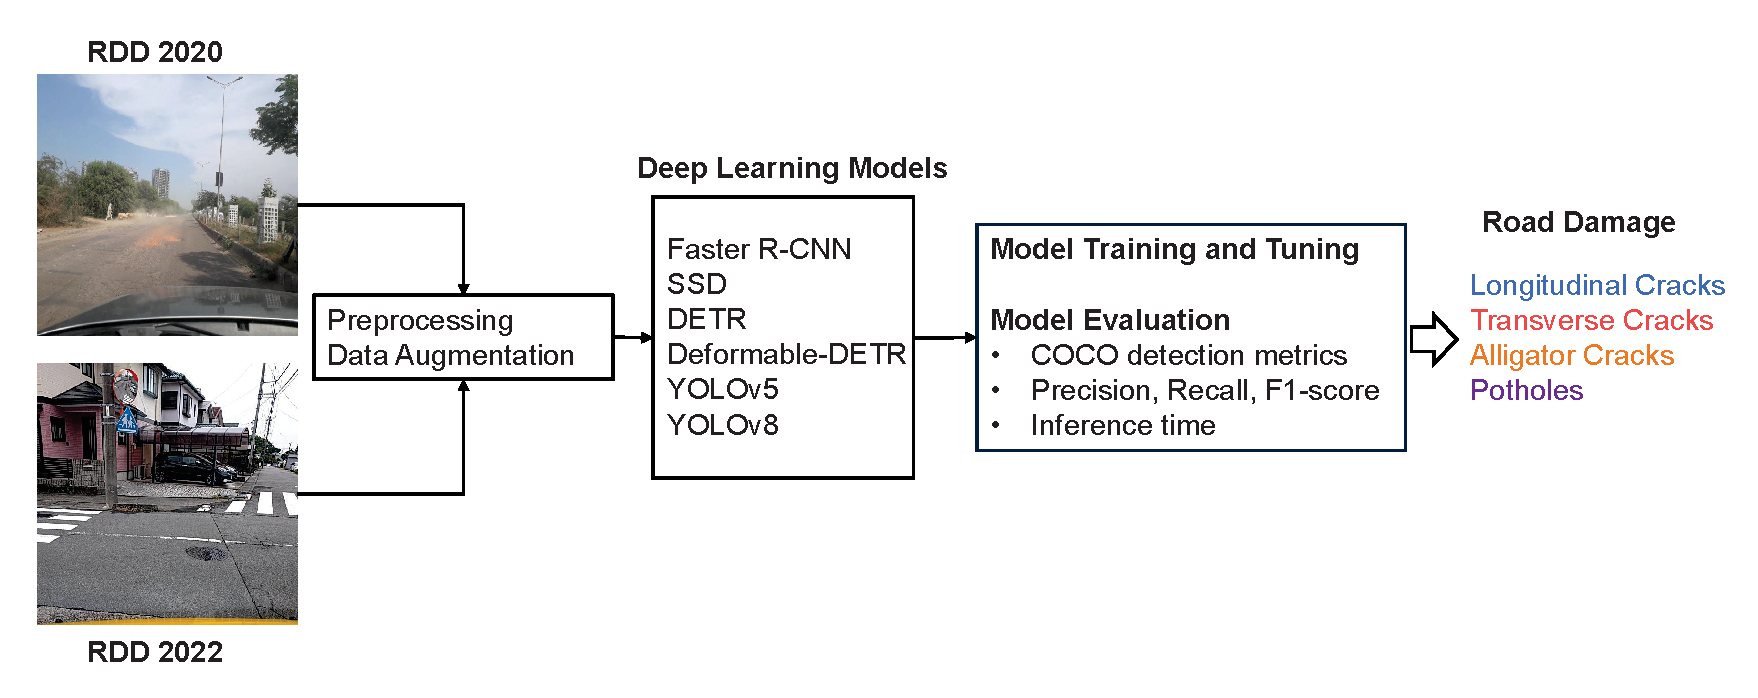
\includegraphics[width=0.95\textwidth]{figs/Figure_overview.eps}
% \end{graphicalabstract}

%%Research highlights
% \begin{highlights}
% \item Comprehensive evaluation of six state-of-the-art object detection models
% \item In-depth comparison of models using two public datasets in detecting road damages
% \item Outline challenges and limitations of datasets, models, and real-world deployments
% \item Future research roadmap for automated road damage detection through critical insights 
% \end{highlights}

% \begin{keyword}
% %% keywords here, in the form: keyword \sep keyword
% Pavement damages \sep automated road maintenance \sep deep learning \sep computer vision \sep road damage detection
% %% PACS codes here, in the form: \PACS code \sep code
% %\PACS 0000 \sep 1111
% %% MSC codes here, in the form: \MSC code \sep code
% %% or \MSC[2008] code \sep code (2000 is the default)
% %\MSC 0000 \sep 1111
% \end{keyword}

% \end{frontmatter}

%% \linenumbers

%% main text
\sloppy
\section{Introduction}

Road transport infrastructure is essential for any modern society and serves as the backbone of economic growth and development \cite{rojo2018impact}. It provides access to critical services and is a crucial component for moving goods, services, and markets. However, factors such as budgetary constraints, underinvestment in upgrades, and delayed maintenance can lead to the degradation of road infrastructure \cite{gopalakrishnan2018deep}. Furthermore, the recent increase in the number of vehicles has also resulted in pavement distress \cite{chen2016development}. Damaged roads cause ecological, economic, and social damage, such as the high costs of vehicle repairs, traffic congestion, accidents, time delays, and additional fuel consumption and emissions \cite{han2020intelligent}. 

Due to the nature of road infrastructure, it is exposed to various types of damage and deterioration, which can be caused by different factors such as traffic load, structural materials, environment, weather, aging, and construction activities \cite{bhandari2023understanding, arya2021deep}. These factors affect the condition and longevity of the pavement. Among these factors, traffic load has a significant influence on pavement performance and causes difficulties in maintaining pavement service life. Therefore, it is essential to maintain the road infrastructure in good condition to ensure the safety of road users and minimize the cost of maintenance.

Pavement damage is an essential aspect of maintaining road infrastructure. There are different ways to evaluate pavement conditions. The evaluation process can be manual, semi-automated, or fully automated \cite{arya2021deep}. Manual pavement condition evaluation is performed by visually inspecting the road surface by trained personnel, which is time-consuming and costly. The manual approach also raises some safety concerns, requiring the person to be on the road surface. Semi-automated evaluation involves taking images of the road surface from a vehicle-mounted camera and evaluating it at a later time to determine the condition of the pavement \cite{zalama2014road, pierce2013practical}. This approach is safer and more efficient compared to the manual process, as it does not require the person to be on the road surface. However, the processing of the images is still done manually, which is time-consuming. Fully automated pavement condition evaluation involves sophisticated sensors such as laser scanners, road profilers, Light Detection and Ranging (LiDAR), and high-resolution cameras that can be used to capture intricate details of the road surface to determine the condition of the surface \cite{eisenbach2017get, guan2021automated}. However, these sensors are costly and difficult to deploy on a large scale.

Recent developments in mobile devices have made it inexpensive to capture images of the road surface using a vehicle-mounted mobile device and process the images using computer vision techniques to determine the condition of the pavement \cite{mertz_city, varadharajan_vision}. This provides a cost-effective and efficient approach to assessing the state of the pavement distress. Arya \etal \cite{arya_grddc20, arya2021deep} have explored the efficacy of combining training data from different sources to achieve better results in the detection problem of road damage. More recently, the Road Damage Detection (RDD) 2022 dataset \cite{arya_rdd2022} was introduced, which is a richer dataset that contains images of road surfaces from different countries around the world. This dataset allows further research to explore the efficacy of training deep learning models using data from other sources.

Several research challenges need to be addressed to achieve a robust and reliable solution to the problem of road damage detection. Due to the nature of the different damages and cracks on the road surface, the target objects to be detected are unique and specific to the problem of detecting road damage. Therefore, selecting an appropriate and efficient deep learning model is crucial to achieving good results. In this article, we present a comprehensive review of state-of-the-art deep learning models for detecting road damage. We provide an in-depth analysis using various performance metrics and comparisons. We also provide key findings, limitations, and future directions. Our key contributions include:
\begin{enumerate}[noitemsep,topsep=0pt]
    \item \textbf{Comprehensive Evaluation of Existing Deep Learning Models}: We have implemented six state-of-the-art deep learning models on the RDD 2022 \cite{arya_rdd2022} and RDD 2020 \cite{arya_grddc20} datasets. Through rigorous experiments, we provide a detailed performance comparison for road damage detection, highlighting their strengths and weaknesses under different scenarios.

    \item \textbf{Deeper insights on challenges and limitations}: In this research, we systematically unveil specific challenges and limitations in current datasets, model-specific restraints, and operational challenges in real-world deployments that can impede the performance of deep learning models. These insights will pave the way for the creation of more robust and comprehensive datasets in the future.
    
    \item \textbf{Future Research Roadmap}: We provide a clear direction for future research to guide researchers in developing more effective models, improving the quality of datasets, exploring diverse model architectures, considerations for lightweight models, integration with inspection systems, and addressing unexplored challenges in the domain.
\end{enumerate}

These insights will help develop practical solutions for future road damage detection applications. Our findings represent a significant step toward streamlining and improving automated road damage detection mechanisms.

% Research Gaps / Limitations of Existing Research:
% on RDD-2020 and RDD-2022 dataset , they mostly discuss older models such as FasterRCNN, SSD, and YOLOv3/v5 etc which are outdated detection models. The existing literature doesn't do an extensive study on the performance and evaluation characteristics and an extensive study of the dataset and results analysis. They mainly report the overall F1-score of the models across different countries and it is difficult to gain a deeper understanding of the performance of the models from this metric alone.

% Besides that, More recently Modified versions of YOLO - YOLOv10 and various Detection Transformers such as DETR, Deformable DETR, DINO, RT-DETR etc. have gained popularity. 

% Our contribution is performing extensive evaluation and validation of different state of the art detection models. It is the first time Detection Transformers have been applied for road damage detection. We apply state of the art versions of YOLO (up to YOLOv10) to obtain the results, do comprehensive validation in terms of mean Average Precision values at different IoU thresholds and for objects of different sizes, and we also report class wise detection metrics such as precision, recall, F1 score, AP. This allows us to better analyze the observed effects across different classes and deep learning architectures. These are our key findings from the study: 


\section{Related Work}

The problem of automated damage detection in road infrastructure has recently garnered a lot of attention thanks to advances in the field of computer vision and deep learning. In this section, we review the existing literature on this topic and discuss the various methods that have been proposed. Specifically, we will discuss traditional methods and recent advancements in deep learning techniques, such as convolutional neural networks and vision transformers. 

\subsection{Traditional Methods}

Traditionally, road damage detection has been approached using image processing techniques and various feature extraction methods, followed by the application of machine learning classifiers. Traditional methods for road crack detection, such as those described in \cite{gavilan_pavement} and \cite{zalama_gabor}, are often expensive and time-consuming, requiring the use of specialized vehicles equipped with line scanners, laser illumination, and
inertial profilers to capture images of the pavement. However, traditional image processing techniques that rely on the assumption that distressed pixels are usually darker than their surroundings (as described in \cite{wang2007positioning}  and \cite{tsai_pavement}) face several challenges, including the effects of different weather conditions, noise, shadow, and the presence of lane markings in images. To address these issues, researchers have proposed a range of pre-processing techniques, including geodesic shadow removal (as described in
\cite{zou_cracktree}), detection of lane markings (\cite{nguyen_pavement}), and various filtering and morphological operations (\cite{huidrom_road, radopoulou_defect,li_pavement}).

Gavlian \etal \cite{gavilan_pavement} extracted features such as the Gray-Level Co-occurrence Matrix (GLCM), Maximally Stable Extremal Regions (MSER), and Local Binary Patterns (LBP) from pavement images. They then used machine learning techniques, including Support Vector Machines and seed-based approaches, to classify the types of pavement distress. The CrackTree algorithm \cite{zou_cracktree} also uses a seed-based system, employing tensor voting to create crack maps from which seeds are sampled and represented in a graph model. Mertz \etal \cite{mertz_city} implemented a smartphone-based system mounted on a vehicle to collect images of damaged roads. Varadharajan \etal \cite{varadharajan_vision} then used these images to perform automated road surface inspection. Their approach involves ground-plane segmentation followed by texture-based superpixel segmentation. They trained a weakly supervised multiple instance learning Support Vector Machine (SVM) to classify surface cracks based on features such as color, location, and texture, which were extracted from the superpixels. Other algorithms for crack detection have been developed based on statistical characteristics, such as those described in \cite{tsai_pavement}, \cite{koutsopoulos_primitive}, and \cite{zhou_wavelet}.

\subsection{Deep Learning Methods}

Traditional methods for detecting road damage can be complex and costly and often struggle to handle challenging scenarios and generalize to different weather and environmental conditions. On the contrary, deep learning has emerged as a promising alternative for road damage detection and object detection tasks. State-of-the-art deep learning methods for object detection include convolutional neural networks (CNNs) and vision transformers, which have demonstrated superior performance on various benchmarks. In the following sections, we discuss these methods in detail.

\subsubsection{Convolutional Neural Networks}

The development of convolutional neural networks (CNNs) has led to the creation of several deep-learning approaches for object detection. One of the first approaches is the Region-Based Convolutional Neural Network (R-CNN) \cite{girshick_rcnn} family, which involves extracting regions of interest (ROIs) from an image using selective search and then classifying each ROI using a CNN. This approach was later improved with the Fast R-CNN algorithm \cite{girshick_fast}, which introduced the use of a region proposal network (RPN) to generate ROI, and the Faster R-CNN algorithm \cite{ren_faster}, which further optimized the process. In addition to these two-stage approaches, single-stage object detection techniques such as the single shot detector (SSD) \cite{liu_ssd} and You Only Look Once (YOLO) \cite{redmon_yolo} algorithms have been proposed. These approaches use a single CNN to predict object classes and locations directly rather than using a separate stage for ROI extraction.

Zhang \etal \cite{zhang_crack} were among the first to apply deep convolutional neural networks (CNNs) to road crack detection, proposing a CNN to classify image patches as containing cracks or not. Gopalkrishnan \etal \cite{gopalkrishnan_transfer} used a deep CNN of Visual Geometry Group (VGG-16) pre-trained to extract features from images of pavement surfaces and various machine learning classifiers to classify pavement distress. Maeda \etal \cite{maeda_rdd2018} introduced a large-scale dataset of road damage images captured with smartphones from seven municipalities in Japan and used the SSD architecture \cite{liu_ssd} for damage detection and classification. This dataset was introduced for the IEEE BigData Cup Challenge 2018, and various researchers proposed solutions for the challenge using deep learning techniques. Other proposed solutions include the Faster R-CNN algorithm and data enhancement techniques \cite{wang_faster_rcnn}, the YOLO \cite{redmon_yolo} object detection algorithm \cite{alfarrarjeh_rdd}  modified YOLO-v2 \cite{redmon_yolov2} architecture \cite{mandal_crack} and RetinaNet \cite{lin_retinanet} for damage detection \cite{ale_retinanet}. 

Bang \etal \cite{bang_encoder} introduced deep convolutional encoder-decoder networks for pixel-level segmentation of road cracks. Maeda \etal \cite{maeda_gan} also proposed a method to generate images of road damage with a Generative Adversarial Network (GAN) and Poisson bleeding to improve the accuracy of damage detection. Arya \etal \cite{arya_multiple} introduced the RDD 2020 dataset \cite{arya_grddc20} from three different countries (Japan, India, and Czech) with four types of damage categories. Recently, the RDD 2022 dataset \cite{arya_rdd2022} has also been introduced to the research community as part of the Crowd Sensing-Based Road Damage Detection Challenge (CRDDC 2022) with data from six countries (Japan, India, Czech, Norway, United States, and China), containing 38,385 images. 


\subsubsection{Vision Transformers}
Vision Transformers (ViTs) \cite{han2022survey} is a type of deep learning model developed built upon the transformer architecture \cite{vaswani_attention}, which was initially created for natural language processing tasks. The transformer architecture introduced the use of self-attention mechanisms, which allow the model to consider relationships between input sequences in a flexible manner. This ability to manage multiple regions of the input simultaneously makes it particularly well suited for tasks that require understanding the relationships between different parts of the information, such as detecting road damage. ViTs were developed by adapting the transformer architecture for use with image data and have shown promising results for a variety of computer vision tasks, including image classification and object detection. In addition to their ability to capture long-range dependencies and handle significant global variations in the data, ViTs also offer other benefits over traditional convolutional neural networks (CNNs), such as the ability to process inputs of variable size and the ability to incorporate additional context from other modalities easily.

Incorporating transformer architectures into deep learning models for structural health monitoring tasks, such as crack detection, has gained attention in recent years. Xiang \etal \cite{xiang_yoloT} implemented transformers in the YOLOv5 architecture \cite{yolo_v5} for this purpose. Xu \etal \cite{xu_letnet} developed an architecture called LetNet that uses a locally enhanced transformer network to detect cracks in pavement images from Charge-Coupled Device (CCD) cameras. Furthermore, Guo \etal \cite{guo_transformer} proposed a model called Crack Transformer (CT) that uses the Swin Transformer \cite{liu_swin} architecture for crack segmentation. These approaches highlight the potential of transformer architectures for crack detection tasks.

\section{Methods}
In this section, we provide an overview of the datasets, data preparation, road damage detection architectures, deep learning training procedure, model evaluation, and specific implementation details. We have implemented six state-of-the-art deep learning models on the RDD 2022 \cite{arya_rdd2022} and RDD 2020 \cite{arya_grddc20} datasets. Figure \ref{fig:overview} gives an overview of our analysis. 

\begin{figure*}[!ht]
    \centering
    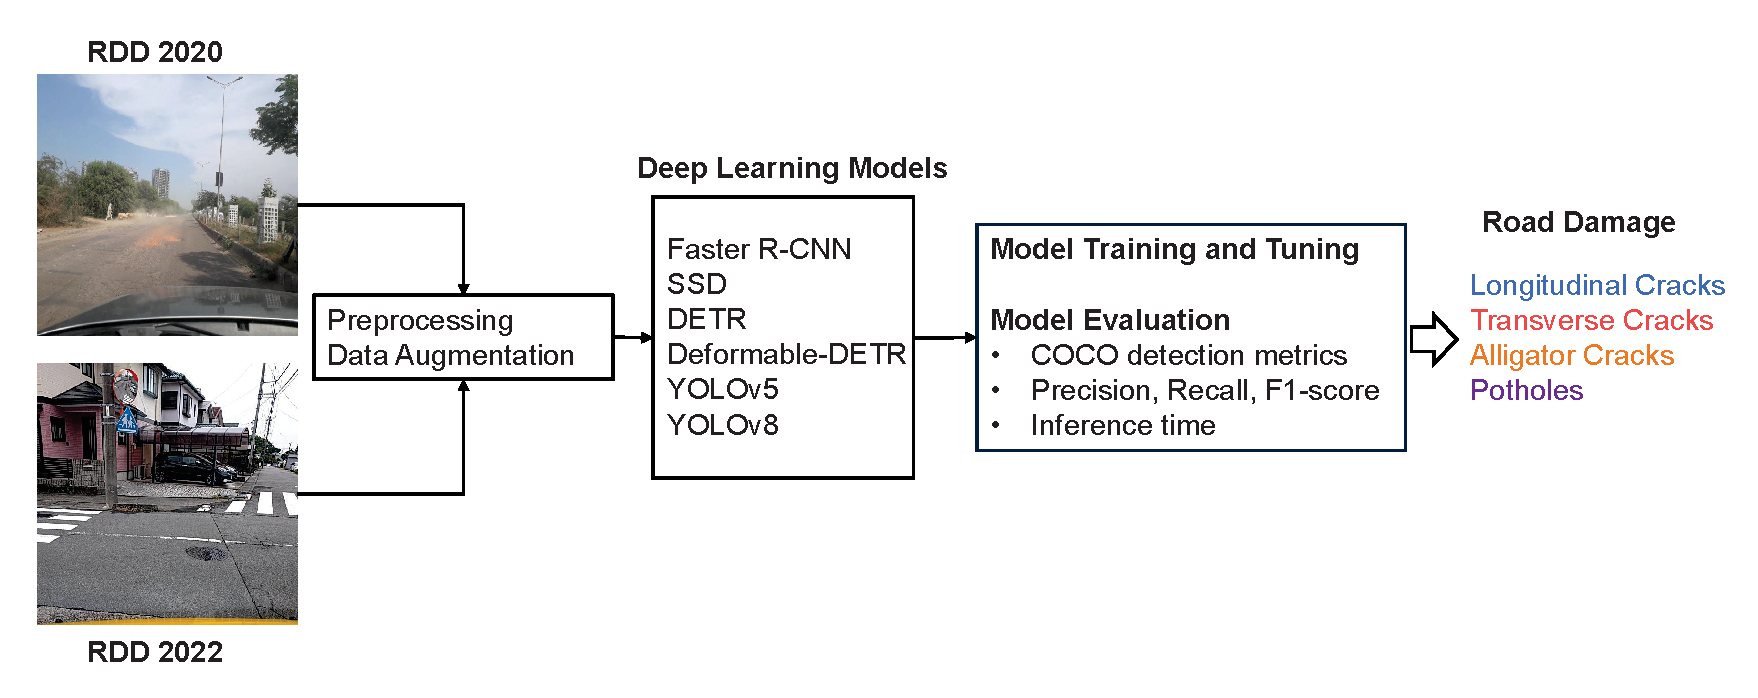
\includegraphics[width=0.9\textwidth]{figs/Figure_overview.eps}
    \caption{An overview of our automated road damage detection framework. We have considered two public datasets (RDD-2020 \cite{arya_grddc20} and RDD-2022 \cite{arya_rdd2022}. In this analysis, we have performed performance comparisons of six state-of-the-art deep learning models (Faster-RCNN \cite{ren_faster}, SSD with MobileNet backbone \cite{liu_ssd}, YOLOv5 \cite{yolo_v5}, YOLOv8, DETR \cite{carion_detr}, and Deformable DETR \cite{zhu_deformable_detr}). We use COCO detection metrics, precision, recall, F1 score, and inference times to elicit deeper insights and future research directions. In this work, we have considered four common types of damages (longitudinal cracks, transverse cracks, alligator cracks, and potholes).} \label{fig:overview}.
\end{figure*}

\subsection{Dataset}
The RDD-2022 dataset \cite{arya_rdd2022} has undergone significant changes over the years to improve its accuracy and extend its applicability to more countries. The original RDD-2018 dataset was introduced in 2018 \cite{maeda_rdd2018} and contained 9,053 road images with 15,435 instances of road damage. Later, the RDD-2018 dataset was used for the 2018 Road Damage Detection Challenge, in which 59 teams from 14 countries participated. However, the dataset was imbalanced, and suggestions were made to improve the annotation files. These suggestions were considered when RDD-2019 was introduced \cite{maeda_gan}, which corrected the annotations and augmented the dataset using generative adversarial networks (GAN). RDD-2019 included 13,133 images with 30,989 instances of road damage.

In 2020, an updated RDD-2020 dataset \cite{arya_grddc20} was introduced to extend the applicability of the models to more countries. The RDD-2020 dataset was formed by combining RDD-2019 with newly collected data from India and the Czech Republic. The RDD-2020 dataset included four damage categories: Longitudinal Cracks, Transverse Cracks, Alligator Cracks, and Potholes. The RDD-2020 dataset was used for the Global Road Damage Detection Challenge (GRDDC-2020), which invited researchers to propose a single model to monitor road conditions in India, Japan, and the Czech Republic with 21,041 images. The best-performing model achieved an F1 score of 0.67 using the YOLOv5-based ensemble model.

The RDD-2022 dataset has been introduced as part of the Crowd Sensing-based Road Damage Detection Challenge (CRDDC-2022) \cite{arya_rdd2022} to solve road damage detection for a more extensive set of countries, including India, Japan, the Czech Republic, Norway, China, and the United States with a total of 38,385 images released for the public. See Table \ref{tab:datasets} for more details on the RDD-2020 and RDD-2022 datasets. 

\begin{table*}[!ht]
\centering
\caption{Details of two public datasets (RDD-2020 \cite{arya_grddc20} and RDD-2022 \cite{arya_rdd2022}) used in this study.}
\label{tab:datasets}
\renewcommand*{\arraystretch}{1.15}
\begin{threeparttable}
\scriptsize
\setlength{\tabcolsep}{3pt}
\begin{tabularx}{\textwidth}{>{\raggedright\arraybackslash}p{1.35cm}>{\raggedright\arraybackslash}p{2.2cm}>{\raggedright\arraybackslash}p{2.2cm}>{\raggedright\arraybackslash}p{1.5cm}>{\raggedright\arraybackslash}p{1cm}>{\raggedright\arraybackslash}p{1.8cm}>{\raggedright\arraybackslash}p{0.95cm}>{\raggedright\arraybackslash}p{0.95cm}>{\raggedright\arraybackslash}p{0.95cm}>{\raggedright\arraybackslash}p{0.95cm}>{\raggedright\arraybackslash}p{0.95cm}}
\hline \hline
Dataset & Countries & Devices & Vehicles & Images & Resolution & Labels & D00 & D10 & D20 & D40  \\ \hline
RDD 2020 & Japan, \newline India,  \newline Czech & Smartphones & Cars & 21,041 & 600 $\times$ 600,   \newline 720 $\times$ 720 & 25,046 & 6,592 & 4,446 & 8,381 & 5,627 \\ \hline
RDD 2022 & Japan,  \newline India,  \newline Czech,  \newline Norway,  \newline United States,  \newline China (drones),  \newline China (motorbikes) & Smartphones, \newline Cameras, \newline Google Street View images & Cars, \newline Motorbikes, \newline Drones & 38,385 & 512 $\times$ 512,  \newline 600 $\times$ 600, \newline 720 $\times$ 720,  \newline 3650 $\times$ 2044 & 55,007 & 26,016 & 11,830 & 10,617 & 6,544  \\ \hline \hline
\end{tabularx}%
\begin{tablenotes}
    \small{
    \item D00: longitudinal cracks; D10: transverse cracks; D20: alligator cracks; D40: potholes
    }
\end{tablenotes}
\end{threeparttable}
\end{table*}

\subsection{Data Preparation}
The RDD-2022 \cite{arya_rdd2022} dataset is in PASCAL VOC format\footnote{http://host.robots.ox.ac.uk/pascal/VOC/}. However, to make it more compatible with the latest object detection techniques, we converted the annotations to the Common Objects in Context (COCO)\footnote{\url{https://cocodataset.org/\#home}} format. To focus on the specific types of road damage that are of particular interest, images from four damage classes were selected and filtered from the dataset. The four damage classes include longitudinal cracks (D00), transverse cracks (D10), alligator cracks (D20), and potholes (D40). 

It is essential to ensure that a deep learning model is trained on a diverse set of images and can generalize well to new, unseen data. To prepare the data for training and testing, a train-test split was performed. This involved random selection of 10\% of the data available from each country as a holdout set (test). The remaining data were split 90:10 for training and validation while maintaining class balance. 
%During modeling training, it was discovered that the choice of data used in the train-test split was critical.
%The model performed poorly when the data were split country-wise, likely due to poor generalizability. Therefore, it was essential to balance the data selection to ensure the model could generalize well to new, unseen data from different countries. 

\subsection{Detection Architectures}

The experiments tested the performance of four different deep-learning network architectures for object detection. These architectures were Faster-RCNN \cite{ren_faster}, SSD with MobileNet backbone \cite{liu_ssd}, YOLOv5 \cite{yolo_v5}, YOLOv8, DETR \cite{carion_detr}, and Deformable DETR \cite{zhu_deformable_detr}. The architectures are briefly described as follows:


\textbf{Faster R-CNN} \cite{ren_faster} architecture is a popular choice for object detection tasks. It consists of two main components: a region proposal network (RPN) and a detection network. The RPN generates candidate object regions that are then passed to the detection network for classification and regression of the bounding box. In our study of road damage detection using computer vision models, we chose the Faster R-CNN architecture with an RPN based on the ResNet50-FPN (Feature Pyramid Network) backbone. ResNet50-FPN combines the ResNet50 architecture with a feature pyramid module \cite{fpn_lin} to effectively capture multi-scale features. This choice enables accurate object localization and improves the model's ability to handle variations in road damage instances. Faster R-CNN with ResNet50-FPN has been widely adopted in various computer vision applications and offers a strong foundation for our road damage detection study.

\textbf{Single Shot MultiBox Detector (SSD)-MobileNet} \cite{liu_ssd} is a single-stage CNN architecture to achieve high detection accuracy with real-time processing speed. For our study on road damage detection using computer vision models, we employ SSD-MobileNet, where MobileNet serves as the base network for feature extraction. We used MobileNetv3 \cite{mobilenetv3_howard} for our implementation, a lightweight convolutional neural network architecture designed for mobile and embedded vision applications. SSD-MobileNet applies convolutional layers of different scales to capture objects at multiple resolutions. Each layer predicts a set of bounding boxes and class probabilities at different scales, resulting in a multi-scale feature map.

% \subsubsection{YOLO-Based Detectors}
\textbf{YOLOv5.} YOLO detectors \cite{redmon_yolo} have played an essential role in advancing object detection techniques. They employ a unique architecture that combines high detection accuracy with real-time inference speed. The original YOLO architecture revolutionized object detection by introducing a single-stage approach that directly predicts bounding boxes and class probabilities using a unified neural network. This eliminated the need for region proposal networks and postprocessing steps, resulting in faster inference times. Over time, several iterations and improvements have been made to the YOLO architecture, leading to the development of different versions of the YOLO model. YOLOv5 \cite{yolo_v5} is a notable advancement in the YOLO series. It consists of convolutional layers followed by upsampling and concatenation operations. YOLOv5 employs anchor boxes and predicts bounding box offsets and objectness scores for each anchor. It has gained popularity because of its simplicity, speed, and competitive performance on various object detection benchmarks. YOLOv5 offers a trade-off between accuracy and efficiency, making it well-suited for real-time road damage detection tasks. We use YOLOv5X in this work.

\textbf{YOLOv8} is an extension of the YOLOv5 architecture based on advances in network design and training strategies. It introduces the  (Coarse to fine) module, which replaces CSPLayer (Cross Stage Partial), effectively combining high-level features with contextual information to improve detection accuracy. Using an anchor-free model with a decoupled head, YOLOv8 allows independent processing of objectness, classification, and regression tasks, improving overall accuracy. The YOLOv8 output layer adopts the sigmoid activation function for the objectness score, indicating the probability of a bounding box containing an object. In contrast, class probabilities are computed using the softmax function.

Furthermore, YOLOv8 incorporates the CIoU (Complete Intersection over Union) and DFL (Distribution Focal Loss) loss functions for bounding-box loss, enabling better performance detecting smaller objects and employing binary cross-entropy for classification loss. With its real-time processing speed and enhanced detection capabilities, YOLOv8 proves to be a promising choice for real-time road damage detection tasks that prioritize both accuracy and efficiency. We use YOLOv8X in this work.

% \subsubsection{Detection Transformers}
\textbf{Detection Transformer} (DETR) \cite{carion_detr} is a recent object detection architecture that replaces traditional two-stage detectors with a transformer-based framework. It models object detection as a direct set prediction problem, where a convolutional backbone processes the input image, and a transformer encoder-decoder architecture generates the final set of bounding box predictions and class probabilities. DETR benefits from the attention mechanism of transformers, which allows it to capture global dependencies between objects efficiently. It has shown promising results in object detection tasks and offers potential advantages for road damage detection by leveraging its ability to handle complex spatial relationships between damage instances.

\textbf{Deformable-DETR} \cite{zhu_deformable_detr} is an extension of DETR incorporating deformable convolutional layers. Deformable convolutions allow the network to adaptively adjust the sampling locations of convolutional kernels, enabling better modeling of geometric variations in objects. Integrating deformable convolutions and multi-scale features into the DETR architecture, Deformable-DETR improves the localization accuracy and robustness of object detection while reducing computational complexity and training convergence times. This makes it well suited for road damage detection, where precise localization of damage instances is crucial.

\begin{table*}[!t] 
\centering  
\renewcommand*{\arraystretch}{1.2}
\caption{Object detection models implemented and evaluated in this work, including optimization algorithms, loss functions, and hyperparameter settings.}
\label{table:models}
\begin{threeparttable}
\scriptsize
\setlength{\tabcolsep}{4pt}
\begin{tabularx}{\textwidth}{>{\raggedright\arraybackslash}p{1.8cm}>{\raggedright\arraybackslash}X>{\centering\arraybackslash}p{1.2cm}>{\raggedright\arraybackslash}p{1.7cm}>{\raggedright\arraybackslash}p{1.4cm}>{\centering\arraybackslash}p{0.9cm}>{\centering\arraybackslash}p{0.9cm}>{\centering\arraybackslash}p{1.05cm}}
\toprule
\textbf{Model} & \textbf{Description} & \textbf{Optimizer} & \textbf{Loss Function} & \textbf{Augmentation} & \textbf{LR} & \textbf{Epochs}& \textbf{Batch Size}\\
\midrule
Faster R-CNN \cite{ren_faster}  & ImageNet \cite{imagenet_deng} pre-trained ResNet50-FPN backbone with Faster-RCNN detection head & SGD & Classification + Localization loss & Horizontal flips & 0.0001 & 30 & 4 \\
SSD-MobileNet \cite{liu_ssd} & ImageNet \cite{imagenet_deng} pre-trained MobileNet-v3-large backbone with single-shot detector & SGD & Classification + Localization + Objectness loss & Flips + crops & 0.001 & 300 & 4 \\
YOLOv5X \cite{yolo_v5} & Modified YOLO architecture with CSPDarkNet53 backbone & Adam & Compound loss & Various & 0.001 & 30 & 16 \\
YOLOv8X \cite{yolov8} & Extension of YOLOv5, introduces C2f module & Adam & CIoU + DFL loss & Advanced & 0.001 & 100 & 16 \\
DETR \cite{carion_detr}  & Detection Transformer with ResNet50 CNN backbone for feature extraction & AdamW & Set loss & Standard & $1\times10^{-5}$ & 300 & 16 \\
Deformable DETR \cite{zhu_deformable_detr} & Extension of DETR with deformable convolution layers & AdamW & Set loss & Standard & $2\times10^{-4}$ & 50 & 4 \\
\bottomrule
\end{tabularx}
\begin{tablenotes}
    \small {
    \item{SGD: Stochastic Gradient Descent}
    \item CIoU: Complete intersection over union
    \item DFL: Distribution Focal Loss
    \item C2f: Cross-Stage Partial bottleneck with two convolutions}
\end{tablenotes}
\end{threeparttable}
\end{table*}

\subsection{Implementation Details}
The Faster R-CNN and SSD models were implemented using the PyTorch deep learning framework. DETR and Deformable-DETR models (based on the transformer architecture) were implemented using the original PyTorch implementations (PyTorch 2.0, Python 3.9, CUDA 11.7). YOLO-based models (YOLOv5X and YOLOv8X) were implemented using the ultralytics\footnote{https://github.com/ultralytics} framework. All models were trained on a high-performance computing (HPC) cluster featuring Nvidia A100 GPUs, and a single A100 GPU was placed in a Linux environment (Red Hat Enterprise 9 based on Fedora).

The details of the training process for each model, including optimization algorithms, loss functions, and hyperparameter settings, are summarized in Table \ref{table:models}. This table provides an overview of the learning rate, batch size, number of epochs, and other vital parameters used during training for each model architecture. 


Model evaluation is a critical step in assessing the performance and effectiveness of object detection models. In this subsection, we discuss the performance metrics used to evaluate the models and the evaluation protocols followed for the evaluation.

\subsubsection{Evaluation Metrics}
\label{sec:metrics}

During the evaluation of object detection models, various metrics are commonly used to assess their performance rigorously. These metrics provide valuable information on different aspects of model performance, including precision, recall, average precision, and the trade-off between precision and recall. The following evaluation metrics were utilized in our analysis:

\begin{enumerate}
  \item \textbf{Intersection over Union (IoU):} The IoU metric measures the overlap between the predicted bounding boxes and the ground truth boxes, indicating the accuracy of object localization. It is calculated using the following formula:
  
  \[IoU = \frac{\text{Area of Intersection}}{\text{Area of Union}}\]
  
  \item \textbf{Precision:} Precision denotes the proportion of true positive detections out of all positive detections made by the model. It quantifies the accuracy of the model's predictions and is calculated as follows:
  
  \[Precision = \frac{\text{True Positives}}{\text{True Positives + False Positives}}\]
  
  \item \textbf{Recall:} Recall measures the proportion of true positive detections out of all ground-truth positive instances. It reflects the model's ability to find all relevant objects and is calculated as,   
  \[Recall = \frac{\text{True Positives}}{\text{True Positives + False Negatives}}\]
  
  \item \textbf{F1 Score:} The F1 score is the harmonic mean of precision and recall, providing a single metric to assess the overall performance of the model. It is given by:  
  \[\text{\textit{F1 Score}} = 2 \times \frac{\text{Precision} \times \text{Recall}}{\text{Precision + Recall}}\]

  \item \textbf{Average Precision (AP):} The AP metric quantifies the performance of object detection by measuring the area under the precision-recall curve. It considers the precision values at various recall levels and calculates their average, providing an overall assessment of the model's detection accuracy for a specific IoU threshold.

  \item \textbf{Mean Average Precision (mAP):} The mAP is a widely used metric that calculates the average precision in different IoU thresholds. It provides an overall assessment of the model's performance. The mAP is computed as the mean of the average precision (AP) values obtained at various IoU thresholds.
  
  \item \textbf{COCO-style AP (AP@[IoU thresholds] - [Size categories]):} The COCO-style AP assesses the average precision at predefined IoU thresholds specified by the COCO dataset. It gauges the model's performance across various IoU values, such as 0.5, 0.75, and 0.95, while considering object size categories: small, medium, and large. This metric provides insights into the model's detection accuracy across different object scales and levels of overlap.
  
  \item \textbf{COCO-style AR (AR@[max detections] - [size categories]):} The COCO-style AR metric evaluates average recall at different maximum detections per image, following the definitions of the COCO dataset. It considers the model's object detection performance across different scenarios of top detections per image, considering object size categories: small, medium, and large. This metric provides insights into the model's capability to detect objects under diverse conditions of detection output.
\end{enumerate}

In addition to these evaluation metrics, precision-recall curves are commonly utilized to analyze the model's performance across different confidence thresholds. These curves plot precision against recall, enabling a comprehensive assessment of the precision-recall trade-off and performance characteristics of the object detection models.

\subsubsection{Evaluation Protocol}
During model evaluation, the designated test set is used to evaluate the performance of the models. The test set consists of labeled images with annotated ground-truth bounding boxes, allowing for the comparison of predicted bounding boxes against the ground truth.

To evaluate the models, the following protocol was followed:
\begin{enumerate}[noitemsep,topsep=0pt]
    \item \textit{Input images:} The test set images were fed into the object detection models, and the bounding box predictions were generated for the objects in the images.
    \item \textit{Calculation of the intersection over the union (IoU):} The IoU was calculated between the predicted bounding boxes and the corresponding ground truth boxes to determine the accuracy of object localization.
    \item \textit{Evaluation metrics:} Using IoU values, metrics such as precision, recall, average precision (AP), F1 score, mean average precision (mAP), COCO-style AP and COCO-style AR were calculated to evaluate model performance.
    \item \textit{Precision recall curve:} By varying confidence thresholds, precision and recall values were obtained, which were then used to plot the precision-recall curve.
    \item \textit{Comparative analysis:} Evaluation metrics and precision-recall curves were analyzed to compare the performance of different object detection models and identify the strengths and weaknesses of each approach.
\end{enumerate}


\section{Results and discussion}
In this section, we provide both quantitative and qualitative results.

\subsection{Quantitative Results}
Road damage detection models were evaluated by comparing their performance using object detection metrics, as detailed in Section \ref{sec:metrics}. This evaluation was conducted on the test sets derived from the RDD-2020 and RDD-2022 datasets. Table \ref{tab:results_coco} provides a comprehensive summary of the COCO object detection metrics achieved by the various models in the RDD-2020 and RDD-2022 datasets.

\begin{table*}[!ht]
\caption{Comparison of performance of six state-of-the-art models on RDD-2020 \cite{arya_grddc20} and RDD-2022 \cite{arya_rdd2022} datasets using COCO detection metrics.}
\centering
\label{tab:results_coco}
\begin{adjustbox}{max width=\textwidth}
\begin{threeparttable}
\scriptsize
\setlength{\tabcolsep}{3pt}

\begin{tabular}{@{}lcccccccccccc@{}}
\toprule
Model/Metric    & AP    & AP    & AP    & AP    & AP    & AP    & AR    & AR    & AR    & AR    & AR    & AR \\
                & 0.50  & 0.50  & 0.75  & 0.50  & 0.50  & 0.50  & 0.50  & 0.50  & 0.50  & 0.50  & 0.50  & 0.50 \\
IoU Threshold   & :0.95 &       &       & :0.95 & :0.95 & :0.95 & :0.95 & :0.95 & :0.95 & :0.95 & :0.95 & :0.95 \\
\midrule
MaxDets         & 100   & 100   & 100   & 100   & 100   & 100   & 1     & 10    & 100   & 100   & 100   & 100   \\
\midrule
Area            & all   & all   & all   & small & medium& large & all   & all   & all   & small & medium & large \\
\midrule
 & \multicolumn{12}{c}{Results on the RDD-2020 \cite{arya_grddc20} dataset} \\
\midrule
Faster R-CNN \cite{ren_faster}     & 0.157 & 0.386 & 0.096 & 0.099 & 0.116 & 0.191 & 0.205 & 0.372 & 0.388 & 0.244 & 0.350 & 0.440 \\
SSD \cite{liu_ssd}            & 0.078 & 0.183 & 0.051 & 0.002 & 0.035 & 0.126 & 0.137 & 0.247 & 0.309 & 0.062 & 0.222 & 0.425 \\
DETR \cite{carion_detr}            & 0.197 & 0.452 & 0.148 & 0.116 & 0.139 & 0.251 & 0.239 & 0.428 & 0.524 & 0.295 & 0.473 & \textbf{0.614} \\
Deformable-DETR \cite{zhu_deformable_detr} & 0.197 & 0.460 & 0.142 & 0.127 & 0.146 & \textbf{0.260}  & \textbf{0.256} & 0.438 & 0.484 & 0.307 & 0.439 & 0.574 \\
YOLOv5X \cite{yolo_v5}  & 0.196 & 0.461 & 0.135 & 0.112 & 0.161 & 0.214 & 0.233 & 0.439 & 0.500 & 0.364 & 0.479 & 0.530 \\
YOLOv8X  \cite{yolov8}        & \textbf{0.223} & \textbf{0.488} & \textbf{0.169} & \textbf{0.141} & \textbf{0.177} & 0.253 & 0.25  & \textbf{0.473} & \textbf{0.536} & \textbf{0.423} & \textbf{0.510} & 0.575 \\
\midrule
 & \multicolumn{12}{c}{Results on the RDD-2022 \cite{arya_rdd2022} dataset} \\
\midrule
Faster R-CNN \cite{ren_faster}      & 0.211 & 0.478 & 0.156 & 0.074 & 0.160 & 0.239 & 0.235 & 0.399 & 0.417 & 0.210 & 0.370 & 0.459 \\
SSD \cite{liu_ssd}              & 0.092 & 0.213 & 0.064 & 0.001 & 0.045 & 0.127 & 0.139 & 0.247 & 0.300 & 0.039 & 0.215 & 0.377 \\
DETR  \cite{carion_detr}          & 0.251 & 0.516 & 0.217 & 0.121 & 0.171 & 0.298 & 0.260 & 0.455 & 0.538 & 0.334 & 0.467 & \textbf{0.607} \\
Deformable-DETR \cite{zhu_deformable_detr} & 0.252 & 0.516 & 0.212 & \textbf{0.160} & 0.185 & 0.293 & 0.271 & 0.472 & 0.519 & 0.379 & 0.459 & 0.579 \\
YOLOv5X \cite{yolo_v5}         & 0.275 & \textbf{0.561} & 0.238 & 0.131 & \textbf{0.228} & 0.295 & 0.272 & 0.477 & 0.531 & \textbf{0.399} & 0.501 & 0.557 \\
YOLOv8X \cite{yolov8}         & \textbf{0.281} & 0.547 & \textbf{0.252} & 0.134 & \textbf{0.228} & \textbf{0.303} & \textbf{0.273} & \textbf{0.495} & \textbf{0.547} & 0.389 & \textbf{0.515} & 0.589 \\
\bottomrule
\end{tabular}
\begin{tablenotes}
    \small {
    \item{\textbf{AP}: Average Precision; \textbf{AR}: Average Recall} }
\end{tablenotes}
\end{threeparttable}
\end{adjustbox}
\end{table*}

As seen in Table \ref{tab:results_coco}, a notable performance improvement is evident in all models when switching from the RDD-2020 \cite{arya_grddc20} to the RDD-2022 \cite{arya_rdd2022} datasets. This performance improvement can be attributed to the infusion of additional data from various countries into the RDD-2022 dataset. This underscores the important role of rich and diverse data in improving model performance. Across both the RDD-2020 \cite{arya_grddc20} and RDD-2022 \cite{arya_rdd2022} datasets, YOLOv8 consistently demonstrated superior performance compared to other models, which is reflected in its higher average precision and average recall metrics across different thresholds. The YOLOv5 \cite{yolo_v5}, Deformable-DETR \cite{zhu_deformable_detr}, and DETR \cite{carion_detr} models also closely trail the YOLOv8 model \cite{yolov8} in terms of performance. On the contrary, SSD \cite{liu_ssd} (the most compact model) exhibited sub-par performance in all metrics. This indicates the demand for greater capacity of the model to capture intricate patterns of road damage effectively.

When assessing the performance of road damage detection in various dimensions and scales, a general trend observed is that all models demonstrate respectable performance with larger dimensions of the bounding box, which gradually decreases as smaller sizes are introduced. On this note, the Deformable-DETR model \cite{zhu_deformable_detr} employs deformable convolutions to enhance the detection of more minor damages. On closer inspection of the results, the Deformable-DETR model exhibits significantly better performance with smaller dimensions when compared to other models. However, this advantage does not extend to larger bounding boxes, which reveals a limitation of this model. A slight but notable performance improvement is also observed with the updated YOLOv8 model compared to the YOLOv5 \cite{yolo_v5} model. Although both models exhibit strong performance, the YOLOv8 model \cite{yolov8}  has slightly better performance due to the more efficient architecture. 

Compared with different IoU thresholds for evaluation, the general trend is that the models decrease precision and recall values with increasing IoU thresholds. However, the YOLOv8 model \cite{yolov8} is more tolerant to higher IoU thresholds and maintains a more balanced result across different IoU thresholds. For recall values, both the DETR \cite{carion_detr} and Deformable-DETR \cite{zhu_deformable_detr} models have a higher recall compared to their precision, suggesting that these models are more likely to detect objects but might have more false positives. The YOLOv8 architecture \cite{yolov8}, despite having the highest precision, maintains consistent recall values, making it a more balanced choice. In general, YOLOv8 seems to be the model that performs best, with YOLOv5 \cite{yolo_v5}, Deformable-DETR \cite{zhu_deformable_detr}, and DETR \cite{carion_detr} closely following.

\begin{table*}[!ht]
\centering
\caption{Comparison of performance of six state-of-the-art models for four crack classes. The four road damage classes are longitudinal cracks (D00), transverse cracks (D10), alligator cracks (D20), and potholes (D40). The best results are highlighted in bold text.}
\label{tab:classwise}
\begin{threeparttable}
\begin{tabular}{m{0.1\textwidth}m{0.1\textwidth}m{0.1\textwidth}m{0.1\textwidth}m{0.1\textwidth}m{0.1\textwidth}m{0.1\textwidth}m{0.1\textwidth}}
\toprule
& \multicolumn{7}{c}{Models} \\  % Adjust column header
\cmidrule(l){3-8}

\multirow{2}{*}{\parbox{0.1\textwidth}{Damage Category}} & 
\multirow{2}{*}{\parbox{0.1\textwidth}{Metric}} &
\multirow{2}{*}{\parbox{0.1\textwidth}{Faster-RCNN}} &
\multirow{2}{*}{\parbox{0.1\textwidth}{SSD}} &
\multirow{2}{*}{\parbox{0.1\textwidth}{DETR}} &
\multirow{2}{*}{\parbox{0.1\textwidth}{Deformable DETR}} &
\multirow{2}{*}{\parbox{0.1\textwidth}{YOLOv5X}} &
\multirow{2}{*}{\parbox{0.1\textwidth}{YOLOv8X}}  \\ \\

\midrule
\multicolumn{8}{c}{Results on the RDD-2020 \cite{arya_grddc20} dataset} \\
\midrule
\multirow{4}{*}{D00}
& Precision & 0.3874 & 0.1998 & 0.4058 & 0.4638 & 0.4504 & \textbf{0.4945} \\
& Recall & 0.3947 & 0.2730 & \textbf{0.4774} & 0.4399 & 0.4743 & 0.4212 \\
& F1 Score & 0.3910 & 0.2307 & 0.4387 & 0.4516 & \textbf{0.4620} & 0.4549 \\
& AP & 0.3183 & 0.1420 & 0.3688 & 0.3767 & \textbf{0.4017} & 0.3851 \\
\midrule
\multirow{4}{*}{D10}
& Precision & 0.4186 & 0.1781 & 0.4877 & 0.4555 & 0.4734 & \textbf{0.4911}\\
& Recall & 0.3682 & 0.1955 & 0.4523 & 0.5000 & 0.4455 & \textbf{0.5023} \\
& F1 Score & 0.3918 & 0.1863 & 0.4693 & 0.4767 & 0.4590 & \textbf{0.4966} \\
& AP & 0.3315 & 0.0874 & 0.4101 & 0.4182 & 0.4105 & \textbf{0.4411} \\
\midrule
\multirow{4}{*}{D20}
& Precision & 0.5898 & 0.5540 & 0.5943 & 0.6278 & 0.6443 & \textbf{0.6389} \\
& Recall & 0.5337 & 0.3975 & \textbf{0.6462} & 0.6050 & 0.5750 & 0.6238 \\
& F1 Score & 0.5604 & 0.4629 & 0.6192 & 0.6162 & 0.6077 & \textbf{0.6312} \\
& AP & 0.5542 & 0.4156 & 0.6188 & 0.6047 & 0.6033 & \textbf{0.6613} \\
\midrule
\multirow{4}{*}{D40}
& Precision & 0.3866 & 0.1532 & 0.5113 & 0.5310 & 0.4281 & \textbf{0.5683} \\
& Recall & 0.3797 & 0.1390 & 0.4029 & 0.4421 & \textbf{0.4724} & 0.4153 \\
& F1 Score & 0.3831 & 0.1458 & 0.4506 & 0.4825 & 0.4492 & \textbf{0.4799} \\
& AP & 0.3139 & 0.0550 & 0.3879 & 0.4227 & 0.4094 & \textbf{0.4464} \\
\midrule
\multicolumn{8}{c}{Results on the RDD-2022 \cite{arya_rdd2022} dataset} \\
\midrule
\multirow{4}{*}{D00}
& Precision & 0.5679 & 0.3347 & 0.5665 & 0.5554 & 0.5820 & \textbf{0.6132} \\
& Recall & 0.4906 & 0.2556 & 0.5044 & 0.5288 & \textbf{0.5682} & 0.5010 \\
& F1 Score & 0.5264 & 0.2899 & 0.5337 & 0.5418 & \textbf{0.5750} & 0.5514 \\
& AP & 0.4929 & 0.1999 & 0.4998 & 0.5048 & \textbf{0.5518} & 0.5258 \\
\midrule
\multirow{4}{*}{D10}
& Precision & 0.5415 & 0.3239 & 0.5787 & 0.5767 & 0.6176 & \textbf{0.6691} \\
& Recall & 0.4799 & 0.2995 & 0.5569 & 0.5298 & 0.5333 & \textbf{0.5595} \\
& F1 Score & 0.5088 & 0.3112 & 0.5676 & 0.5523 & 0.5724 & \textbf{0.6094} \\
& AP & 0.4864 & 0.1942 & 0.5497 & 0.5515 & 0.5605 & \textbf{0.5891} \\
\midrule
\multirow{4}{*}{D20}
& Precision & 0.5946 & 0.5622 & 0.6748 & 0.6071 & 0.6436 & \textbf{0.7051} \\
& Recall & 0.5690 & 0.3937 & 0.5862 & \textbf{0.6054} & \textbf{0.6054} & 0.5450 \\
& F1 Score & 0.5815 & 0.4631 & \textbf{0.6274} & 0.6062 & 0.6239 & 0.6148 \\
& AP & 0.5909 & 0.4060 & 0.6323 & 0.6015 & \textbf{0.6404} & 0.6383 \\
\midrule
\multirow{4}{*}{D40}
& Precision & 0.4184 & 0.0849 & 0.4454 & 0.4462 & \textbf{0.5804} & 0.5009 \\
& Recall & 0.3760 & 0.1654 & 0.4009 & \textbf{0.4727} & 0.4446 & 0.4462 \\
& F1 Score & 0.3961 & 0.1122 & 0.4220 & 0.4591 & \textbf{0.5035} & 0.4719 \\
& AP & 0.3272 & 0.0306 & 0.3746 & 0.3957 & \textbf{0.4839} & 0.4286 \\
\bottomrule
\end{tabular}
\begin{tablenotes}
    \small{
    \item AP: Average Precision
    \item D00: longitudinal cracks; D10: transverse cracks; D20: alligator cracks; D40: potholes
    } 
\end{tablenotes}
\end{threeparttable}
\end{table*}

\begin{figure*}[!ht] % 
    \centering 
    \includegraphics[width=0.75\textwidth]{figs/prc_classwise_rdd20.pdf} % Adjust width as needed
    \caption{Precision-Recall curves for the best performing models (DETR \cite{carion_detr}, Deformable DETR \cite{zhu_deformable_detr}, YOLOv5 \cite{yolo_v5} and YOLOv8 \cite{yolov8}) on the RDD-2020 \cite{arya_grddc20} dataset. The best results are highlighted in bold text.}
    \label{fig:prc_rdd20}
\end{figure*}

\begin{figure*}[!ht] % 
    \centering 
    \includegraphics[width=0.75\textwidth]{figs/prc_classwise_rdd22.pdf} % Adjust width as needed
    \caption{Precision-Recall curves for the best performing models (DETR \cite{carion_detr}, Deformable DETR \cite{zhu_deformable_detr}, YOLOv5 \cite{yolo_v5} and YOLOv8 \cite{yolov8}) on the RDD-2022 \cite{arya_rdd2022} dataset.}
    \label{fig:prc_rdd22}
\end{figure*}

Table \ref{tab:classwise} presents the class-wise performance of six state-of-the-art models for the RDD-2020 \cite{arya_grddc20} and RDD-2022 \cite{arya_rdd2022} datasets. We notice trends similar to those observed in the COCO object detection metrics presented in Table \ref{tab:results_coco}, where the introduction to the RDD-2022 \cite{arya_rdd2022} dataset leads to an improvement in the detection scores across the board. Models based on the YOLO architecture exhibit notable performance, leading several class-wise detection metrics. The YOLOv8 model \cite{yolov8} shows the best performance in the RDD-2020 dataset \cite{arya_grddc20} and also shows competitive performance across different classes of the RDD-2022 dataset. Interestingly, despite the advantage of YOLOv8 in COCO mAP metrics (as shown in Table \ref{tab:results_coco}), the YOLOv5 model \cite{yolo_v5} offers better performance in three of the four damage categories within the RDD-2022 dataset. This discrepancy highlights the effect of the class imbalance of the datasets. 

When we look at the difference in performance across various classes, all models tend to have higher precision and an F1 score for the ``D20" damage category (alligator cracks). On visual examination of these cracks, their relatively larger size and distinct features are evident, making them easy to detect by the models. On the contrary, the ``D40" damage category (potholes) is, in general, not only smaller in dimensions but also has fewer samples in the datasets. The limited representation likely poses additional challenges to the models' difficulties in detection, as evidenced by the performance metrics. Regarding the remaining two damage categories, ``D00" (longitudinal cracks) and ``D10" (transverse cracks), all models show comparable performance metrics that align with their similarity in visual characteristics. 

The DETR models exhibit commendable performance in various damage categories, although they slightly trail behind the YOLO models. The introduction to deformable convolution yields exciting results. This architectural tweak improves performance on longitudinal and transverse cracks, as well as potholes while resulting in a performance drop for alligator cracks. This reveals a nuanced impact of architectural changes and also underscores the limitation of Deformable-DETR \cite{zhu_deformable_detr} in the detection of larger cracks. In general, DETR-based models \cite{carion_detr, zhu_deformable_detr} demonstrate strong performance in most damage categories. However, compared to the YOLO models \cite{yolo_v5, yolov8}, they show diminished performance in pothole detection. 

In summary, except SSD \cite{liu_ssd}, all models demonstrate competitive performance in various performance metrics for detecting road damage. The performance of more advanced models based on DETR \cite{carion_detr, zhu_deformable_detr} or YOLO \cite{yolo_v5, yolov8} architectures is particularly notable. Both YOLO models demonstrate versatility and robustness in effectively addressing various crack types.

\subsubsection*{Precision-Recall Curves}

Figures \ref{fig:prc_rdd20} and \ref{fig:prc_rdd22} visually represent the precision-recall curves for the different damage categories within the RDD-2022 \cite{arya_rdd2022} dataset, highlighting the performance of the best performing models (DETR \cite{carion_detr}, Deformable DETR \cite{zhu_deformable_detr}, YOLOv5 \cite{yolo_v5} and YOLOv8 \cite{yolov8}). Depending on the damage category, all models tend to follow a general trend for the precision-recall curves. The precision-recall curves corroborate the insights from Table \ref{tab:classwise}, with the YOLOv5 and YOLOv8 models leading in performance.  

\subsubsection{Confusion Matrices}
\begin{figure*}[!ht] % 
    \centering 
    \includegraphics[width=0.75\textwidth]{figs/confusion_matrix_rdd20.pdf}
    \caption{Normalized confusion matrices, comparing performances of best-performing models (DETR \cite{carion_detr}, Deformable DETR \cite{zhu_deformable_detr}, YOLOv5 \cite{yolo_v5} and YOLOv8 \cite{yolov8}) on the RDD-2020 dataset.}
    \label{fig:conf_rdd20}
\end{figure*}

\begin{figure*}[!ht] %  
    \centering 
    \includegraphics[width=0.75\textwidth]{figs/confusion_matrix_rdd22.pdf}
    \caption{Normalized confusion matrices, comparing performances of best-performing models (DETR \cite{carion_detr}, Deformable DETR \cite{zhu_deformable_detr}, YOLOv5 \cite{yolo_v5} and YOLOv8 \cite{yolov8}) in the RDD-2022 \cite{arya_rdd2022} dataset.}
    \label{fig:conf_rdd22}
\end{figure*}

Confusion matrices were computed for various models using the RDD-2020 \cite{arya_grddc20} and RDD-2022 \cite{arya_rdd2022} datasets. Normalized confusion matrices for the RDD-2020 and RDD-2022 datasets are illustrated in figures \ref{fig:conf_rdd20} and \ref{fig:conf_rdd22}, respectively. A close examination of the confusion matrices shows some interesting patterns, especially in contrast to the class-wise performance metrics documented in Table \ref{tab:classwise}. It is worth mentioning that a global confidence threshold was employed during the computation of the confusion matrices. This approach yields more overarching findings in diverse classes. 

\begin{table*}[!ht]
    \centering
    \caption{Comparison of state-of-the-art models used in this study and their inference time. The best result is highlighted in bold text.}
    \begin{tabular}{lccc}
        \toprule
         \textbf{Model} & \textbf{Input image size} & \textbf{Total model parameters} & \textbf{Average inference time (ms)}\\
         \midrule
         Faster R-CNN & 720 x 720 & 41.3 M & 15.10 \\
         SSD & 720 x 720 & 3.7 M & 8.84 \\
         DETR & 1200 x 800 & 41.5 M & 8.13 \\
         Deformable DETR &  1200 x 800 & 41 M & 22.58 \\
         YOLOv5X & 640 x 640 & 86.1 M & 6.32 \\
         YOLOv8X & 640 x 640 & 68.2 M & \textbf{5.91} \\
         \bottomrule
    \end{tabular}

    \label{tab:inference_time}
\end{table*}

Analyzing the confusion matrices of the RDD-2020 dataset \cite{arya_grddc20}, Deformable-DETR \cite{zhu_deformable_detr} is regarded as the best performer in terms of precision, closely followed by the results of the DETR architecture. However, the YOLOv5 \cite{yolo_v5} and YOLOv8 \cite{yolov8} architectures exhibit vulnerabilities in the detection of inevitable cracks, with the former demonstrating suboptimal performance in the detection of transverse cracks and the latter in the detection of potholes. Turning our attention to the RDD-2022 \cite{arya_rdd2022} dataset, the YOLOv5 \cite{yolo_v5} architecture shows a balanced overall performance. The Deformable-DETR architecture also remains competitive. The DETR \cite{carion_detr} and YOLOv8 architectures perform well in most damage categories, except potholes. 



Across both datasets, a recurring observation is that all models show some weakness in detecting pothole examination. They exhibit strong performance when detecting alligator cracks. The detection precision for longitudinal and transverse cracks is also commendable, with a few exceptions. Considering false positives, a uniform representation of the different damage categories is present for the RDD-2020 \cite{arya_grddc20} dataset. In contrast, the RDD-2022 \cite{arya_rdd2022} dataset is characterized by a rise in false positives for longitudinal cracks, leaving other damage categories with considerably lower false positive rates. Regarding false negatives, potholes consistently register the highest rates, underscoring the challenge of classifying this type of damage. 

A particularly salient observation from both confusion matrices is the models' remarkably low inter-class confusion. In other words, misclassifications across different damage categories are notably rare. This underscores the strengths of the models in distinguishing among types of damage. Our primary focus in the future would be to address and reduce the occurrence of false positives and false negatives. 

\subsection{Inference time}
Table \ref{tab:inference_time} compares the inference times of six state-of-the-art object detection models. Table \ref{tab:inference_time} also provides the input image size of the models and the corresponding number of model parameters. We can see that YOLOv8X has the least inference time (5.91 ms), which is highly suitable for real-time applications, such as road damage detection. We also observe that YOLOv5X is the second best, with an inference time of 6.32 ms.% In a general pattern, we see that the more complex the model is, the more parameters it will have and, therefore, the higher the inference time. For example, the Deformable DETR model is more complex and has a higher inference time (22.58 ms). The exception to this observation is the YOLO family models, which, despite having a more significant number of parameters, their inference times are lower. 
In general, a more complex model equates to a longer inference time, as can be seen with the Deformable DETR. However, it should be noted that the Deformable DETR variant we employed here utilizes special techniques such as iterative bounding box refinement and two-stage detection, which is responsible for the higher inference time. A variant without these modifications should have lower inference times at the cost of performance. The YOLO models, which are purpose-built for real-time applications, on the other hand, have significantly lower inference times due to the simpler architecture despite having a higher parameter count.

\subsection{Qualitative Results}
This section presents a qualitative analysis of different road damage detection models through visual examination of the RDD-2022 \cite{arya_rdd2022} dataset. Since the RDD-2020 dataset is a subset of the RDD-2022 dataset \cite{arya_rdd2022}, the predictions in the RDD-2022 dataset inherently cover the road damage scenarios present in the RDD-2020 dataset. The purpose of this visual analysis is to provide insights into the strengths and limitations of different models' predictions, as well as to explore any discrepancies between the ground-truth annotations and forecasts of the models. A detailed visual examination of the different types of road damage present in the RDD-2020 and RDD-2022 datasets concerning the predictions of the top-performing deep learning models for road damage detection helps us understand the performance of the models conceiving different types of road damage, spatial distribution, and overall prediction precision. This qualitative evaluation complements the quantitative metrics presented earlier, enhancing understanding of the effectiveness of the models.

Figure \ref{fig:det_rdd22} illustrates the road damage predictions of the top performing models, namely DETR \cite{carion_detr}, Deformable DETR \cite{zhu_deformable_detr}, YOLOv5 \cite{yolo_v5}, and YOLOv8 \cite{yolov8}. In general, these models demonstrate strong performance in detecting road damage instances. However, there are isolated cases where specific models struggle to identify road damage. The models collectively exhibit the ability to detect various types of road damage, including longitudinal cracks, transverse cracks, alligator cracks, and potholes, with a notable degree of accuracy.

\begin{figure*}[!ht] % 
    \centering 
    \includegraphics[width=\textwidth]{figs/good-preds/China_Drone_000917.pdf}
    \includegraphics[width=\textwidth]{figs/good-preds/Japan_006122.pdf}
    \includegraphics[width=\textwidth]{figs/good-preds/Japan_009915.pdf}
    \includegraphics[width=\textwidth]{figs/good-preds/United_States_001436.pdf}    
    \caption{\textbf{Road damage predictions} by four best models on the RDD-2022 \cite{arya_rdd2022} dataset. In the figure, each row corresponds to a sample of ground truth damages followed by predictions of DETR \cite{carion_detr}, Deformable DETR \cite{zhu_deformable_detr}, YOLOv5X \cite{yolo_v5} and YOLOv8X \cite{yolov8}.}
    \label{fig:det_rdd22}
\end{figure*}

While investigating the performance of the different models, we encountered an intriguing phenomenon in the behavior of the models, where we observed a considerably high number of false positives, which impacted the overall detection scores. A meticulous examination of the predictions revealed certain cases where the models detected road damages that were not present in the ground-truth annotations but were visually discernible. Such examples are illustrated in Figure \ref{fig:missing_rdd22}. This observation was not isolated, as similar cases were scattered throughout the dataset. 

\begin{figure*}[!ht] % 
    \centering 
    \includegraphics[width=\textwidth]{figs/missing-annots/China_Drone_000524.pdf}
    \includegraphics[width=\textwidth]{figs/missing-annots/India_006463.pdf}
    \includegraphics[width=\textwidth]{figs/missing-annots/Japan_000225.pdf}
    \includegraphics[width=\textwidth]{figs/missing-annots/Japan_006612.pdf}
    \caption{Four best model predictions on images with \textbf{missing annotations} on the RDD-2022 \cite{arya_rdd2022} dataset. In the figure, each row corresponds to a sample of ground truth damages followed by predictions of DETR \cite{carion_detr}, Deformable DETR \cite{zhu_deformable_detr}, YOLOv5X \cite{yolo_v5} and YOLOv8X \cite{yolov8}.}
    \label{fig:missing_rdd22}
\end{figure*}

Moreover, the dataset presented some complex scenarios, such as the coexistence of multiple types of cracks, such as potholes embedded within alligator cracks, or the juxtaposition of linear cracks alongside alligator cracks. A pattern of inconsistency was also noted within the ground truth annotations for these complex scenarios. The combination of these inconsistencies, along with missing annotations, might explain the variable performance of the models when trying to detect road damage from challenging scenarios. The lack of consistent annotations could hinder models from fully discerning the intricate features associated with road damage.

Further investigation revealed distinct behaviors between the models employed. DETR \cite{carion_detr} and Deformable-DETR \cite{zhu_deformable_detr} models exhibited greater generalizability, detecting more instances of road damage that were absent in the ground truth data. On the contrary, the YOLOv5 \cite{yolo_v5} and YOLOv8 \cite{yolov8} models showed better alignment with ground truth data, indicating a possible susceptibility to overfitting. Although the DETR \cite{carion_detr} and Deformable-DETR \cite{zhu_deformable_detr} models demonstrated slightly lower performance in terms of quantitative metrics; their generalizability underscores their potential for robust detection of road damage with improved training data.

\section{Key Findings and Limitations}
In this section, we highlight key insights from our study on the performance of six state-of-the-art models using the RDD-2020 \cite{arya_grddc20} and RDD-2022 \cite{arya_rdd2022} datasets. We delve into the challenges and limitations of the datasets and the different model architectures. We also discuss the broader implications of applying these models in real-world scenarios.

\subsection{Summary of Key Findings}
\begin{enumerate}[noitemsep,topsep=0pt]
    \item \textit{Road Damage Detection Performance:} Our extensive evaluation in the RDD-2020 \cite{arya_grddc20} and RDD-2022 \cite{arya_rdd2022} datasets highlighted the capabilities of the various object detection models for road damage detection. The YOLOv8 model \cite{yolov8} stands out in terms of balanced performance metrics for detection. The Deformable-DETR \cite{zhu_deformable_detr}, YOLOv5 \cite{yolo_v5}, and DETR \cite{carion_detr} models also showed competitive results that reflect their effectiveness in detecting various types of road damage. 
    
    \item \textit{Influence of Diverse Data:} A notable boost in model performance is observed when transitioning from the RDD-2020 \cite{arya_grddc20} to the more diverse RDD-2022 \cite{arya_rdd2022} dataset. This underscores the importance of a rich and varied dataset for the road damage detection task.
    
    \item \textit{Performance Across Damage Categories:} When analyzing the performance of the models against different damage categories, the models showed a strong performance in detecting alligator cracks (``D20'' class) while facing difficulties in detecting more minor damage instances, such as potholes (``D40'' class). Models demonstrated comparably commendable performance detecting linear cracks, such as longitudinal and transverse cracks.
    
    \item \textit{Qualitative Observations:} Visual examination of the models' performance revealed intriguing behaviors of the models such as DETR \cite{carion_detr} and Deformable-DETR \cite{zhu_deformable_detr} actively detected damages not annotated in the ground truth, whereas the YOLOv5 \cite{yolo_v5} and YOLOv8 \cite{yolov8} models showed a closer alignment with the ground truth.
\end{enumerate}

\subsection{Dataset Limitations}
In any deep learning task, the quality of the datasets plays a critical role in the model's performance. However, our close inspection of the RDD-2020 \cite{arya_grddc20} and RDD-2022 \cite{arya_rdd2022} datasets revealed certain limitations that could hinder the effectiveness of object detection models. These are discussed as follows:

\begin{enumerate}[noitemsep,topsep=0pt]
    \item \textit{Annotation inconsistency :} One of the main difficulties in obtaining reliable results from object detection models is the variability in the provided ground truth annotations. A closer examination revealed that this inconsistency is particularly prominent in complex scenarios, such as when multiple types of damage coexist. This situation could potentially lead to confusion during model training.
    \item \textit{Missing annotations:} A detailed analysis revealed that there were instances in which the models detected road damage that was visible but not marked on the ground truth data. This poses a two-fold issue: While on the one hand, it penalizes models for their correct detections as false positives, on the other hand, it can lead to models missing out on learning crucial representations from the missing annotations.
    \item \textit{Class imbalance:} The datasets also exhibited signs of class imbalance. Certain types of damage, such as potholes (``D40''), were underrepresented (11.9\% in the RDD-2022 dataset and 22.5\% in the RDD-2020 dataset) compared to other damage categories in the dataset, and this hurt the detection rates for this damage category.
\end{enumerate}

\subsection{Model-Specific Limitations}
The distinct behaviors exhibited by various models underscore their unique limitations. For example, the SSD \cite{liu_ssd} and Faster R-CNN \cite{ren_faster} models, while more compact, often trail behind in performance compared to their counterparts. 

A particularly intriguing observation emerges when comparing DETR-based models \cite{carion_detr, zhu_deformable_detr} with YOLO-based models \cite{yolo_v5, yolov8}. Although YOLO models \cite{yolo_v5,yolov8} demonstrate better performance metrics and are closely aligned with the ground truth, visual analysis reveals that DETR-based models \cite{carion_detr, zhu_deformable_detr} often detect road damage absent from the ground truth. This suggests that, while efficient YOLO models might be leaning toward overfitting, the more computationally intensive DETR models offer greater generalizability. This presents a compelling trade-off determined by the choice of model and architecture.

The challenges models face in detection of small road damages, such as potholes, emphasize an area of potential improvement. Models such as Deformable-DETR \cite{zhu_deformable_detr}, designed to enhance finer details, exhibited improved performance in detecting smaller damages. However, this came at the cost of lower performance in detecting larger damages. This highlights the need for models that can bridge the gap between small and large damage types without introducing bias. 

\subsection{Operational and Real-world Limitations}
In operational contexts, real-world applications introduce multifaceted challenges for detecting road damage. These challenges are discussed as follows:
\begin{enumerate}[noitemsep,topsep=0pt]
    \item \textit{Complex scenarios:} Road damages frequently manifest as complex scenarios in real-world settings. Roads can exhibit many defects, often overlapping or coexisting nearby. This poses a challenge to models trained to detect isolated damage. For example, a pothole near a crack could be misclassified as a sizeable singular damage. Furthermore, existing datasets may not encompass every possible damage scenario encountered in real-life tests, adding to the challenge of the task. 
    
    \item \textit{Scalability and deployment:} The diversity of road conditions in different geographies makes scaling the models for more extensive deployment challenging. For example, what is considered ``damage'' in one region might be considered normal wear in another. Additionally, differences in road types, such as asphalt or cobblestone, highways, or local roads, also introduce variability. Training a model that encompasses various conditions demands careful curation of the dataset and fine-tuning of the models to reduce the risk of misdetections.
    
    \item \textit{Computational overheads:} Sophisticated models typically perform better in road damage detection tasks but require greater computational power. When considering the need for real-time applications, high-accuracy, resource-intensive models might not be feasible. The associated hardware and energy costs pose challenges in resource-limited settings. Thus, striking a balance between accuracy and computational efficiency becomes crucial in real-world applications. For example, the YOLOv5 and YOLOv8 models (see Table \ref{tab:inference_time}) have a shorter inference time and less computational overhead than other object detection models.
\end{enumerate}

\section{Future Work}

Our research aims to provide meaningful insight into the potential of state-of-the-art object detection models for detecting road damage. However, as with all exploratory studies, our work sets the foundation for numerous avenues for further investigation and research. Some of the areas that we have identified for future exploration are discussed in the following sections. 

\subsection{Dataset Augmentation and Annotation Improvement}

The inconsistencies and missing annotations in the current dataset suggest a clear area for improvement. Future work can focus on: 

\begin{enumerate}[noitemsep,topsep=0pt]
    \item \textit{Curated Data Collection:} Initiating a campaign with trained professionals to curate the annotations and the collected data carefully can vastly improve the quality of the annotations and also reduce the problem of class imbalance.
    
    \item \textit{Enhanced Annotation Techniques:} Deploying semi-automated annotation tools can be utilized to improve the quality of the annotations further.
    
    \item \textit{Generating Synthetic Data:} Employing techniques like Generative Adversarial Networks (GANs) can help diversify underrepresented damage categories such as potholes. Maeda et al. \cite{maeda_gan} used GANs to improve the representation of potholes in the RDD-2019 dataset, resulting in improved detection performance. Applying similar techniques to RDD-2022 could probably improve detection scores.
\end{enumerate}

\subsection{Different Learning Paradigms}

Considering the inconsistencies and missing annotations present in our datasets, there is an opportunity to explore different learning paradigms that leverage incomplete or imperfect data, such as:

\begin{enumerate}[noitemsep,topsep=0pt]
    \item \textit{Semi-Supervised Learning:} Given the instances in which road damage is visible but not annotated, we can apply semi-supervised learning techniques \cite{tang2021proposal,xu2021end}. This strategy effectively leverages both labeled and unlabeled data. 
    
    \item \textit{Active Learning:} This process might contribute to the refinement of the datasets. Through an iterative process of model training and subsequent identification of the most ambiguous cases for human annotators, we can optimize the annotation process while simultaneously improving the accuracy of the model. Recent initiatives such as the Segment Anything Model (SAM) \cite{sam_meta} employ methods such as active learning to achieve notably precise computer vision datasets.
\end{enumerate}

\subsection{Exploration of Model Architectures}

While we have observed promising results with our current object detection models based on DETR and YOLO architectures, there is ample room for several architectural modifications and techniques to be explored:

\begin{enumerate}[noitemsep,topsep=0pt]
    \item \textit{Hybrid Models:} Given the unique challenges of detecting large and small road damage, utilizing hybrid architectures that merge the strengths of various models can be a promising direction.
    
    \item \textit{Architectural tweaks:} Architectural tweaks, such as incorporating multi-scale feature extraction to improve detection of both significant and minor damage, use of attention mechanisms to focus on damage-specific visual patterns, etc., can be explored.
    
    \item \textit{Knowledge Distillation:} To create lightweight and accurate models suited for resource-constrained settings, techniques such as knowledge distillation can be explored.
\end{enumerate}

\subsection{Additional Future Directions}

\begin{enumerate}[noitemsep,topsep=0pt]
    \item \textit{Real-time Detection Systems:} Exploring the development of lightweight and efficient models suitable for real-time road damage detection in mobile or embedded systems.
    
    \item \textit{Geographic Adaptation:} Given the variability in road conditions across regions, design models consider domain adaptation techniques so that models can easily be adapted or fine-tuned for specific geographic conditions.
    
    \item \textit{Integration with Inspection Systems:} The ultimate goal of detecting road damage is a swift and precise inspection that leads to timely repairs. Subsequent efforts could focus on developing tools to seamlessly integrate the model into existing road inspection systems and workflow.
\end{enumerate}

\section{Conclusion}

In our comprehensive study of various state-of-the-art object detection models applied to the RDD-2020 \cite{arya_grddc20} and RDD-2022 \cite{arya_rdd2022} datasets, our objective was to uncover the strengths, limitations, and potentials of these models for road damage detection. While there are many studies on object detection tasks, there remains a notable gap in research that focuses on applying contemporary object detection models for detecting road damage. Our study aims to bridge the gap, presenting the road damage detection performance of an array of deep learning object detection models. Our findings highlight the distinct characteristics, strengths, and weaknesses of different models, including leading architectures based on DETR \cite{carion_detr, zhu_deformable_detr} and YOLO \cite{yolo_v5, yolov8}. The models demonstrated competitive performance on the RDD-2022 dataset for road damage detection. However, our study also underscores the challenges posed by inconsistent annotations, class imbalances, and model-specific behaviors, highlighting the complexities of implementing such models in real-world settings.

Detecting road damages quickly and accurately is critical to ensuring public safety and optimizing the maintenance of transport infrastructure. Our findings represent a significant step toward streamlining and improving automated road damage detection mechanisms. The implications of our research extend beyond academic exploration. The broader impact of our study is the dual potential for cost savings in road infrastructure management, as well as improved public safety. With better detection capabilities, authorities can prioritize and allocate resources more efficiently, ultimately leading to safer roads. 

Our study provides valuable information on the current landscape while paving the way for future endeavors. We are optimistic that this research will be a foundation for future work such as dataset refinement, architectural innovations, etc. As the object detection field continues to evolve, we hope that the groundwork established by this research will promote further innovations and propel us closer to the ultimate goal of a robust and efficient automated road damage detection solution.

% \section*{Acknowledgement}
% This research was supported partially by the Australian Government through the Australian Research Council's Linkage Projects funding scheme (project LP190100079). The views expressed herein are those of the authors and are not necessarily those of the Australian Government or the Australian Research Council.

% \balance
% \bibliographystyle{elsarticle-num} 
% \bibliography{references}



% \end{document}


\chapter{Explainability Analysis of DETRs}
\label{chap:explainability}
% Placeholder content for Chapter 4.
\lipsum[4]


\chapter{MCAF-DETR: Multi-Scale Cross Attention Fusion}
\label{chap:mcaf-detr}
% Placeholder content for Chapter 5.
\lipsum[5]


\chapter{BLCA (Optional): Bidirectional Latent Cross Attention for Efficient DETRs}
\label{chap:blca}
% Placeholder content for Chapter 6.
\lipsum[6]


\chapter{Conclusion}
% Placeholder content for Chapter 7.
\lipsum[7]


% Optional: include appendices for this chapter by uncommenting below.
%\appendix
%\input{Appendices/AppendixA}

\clearpage
\label{Bibliography}
\lhead{\emph{Bibliography}}
\bibliographystyle{unsrtnat}
\bibliography{Bibliography}

\end{document}
